\documentclass[11pt,a4paper]{article}
\usepackage{amsmath}
\usepackage{amsfonts}
\usepackage{amssymb}
\usepackage{fancyhdr}
\usepackage{lastpage}
\usepackage{graphicx}
\usepackage{ucs}
\usepackage[utf8x]{inputenc}
\usepackage[italian]{babel}
\usepackage[colorlinks=true,linkcolor=black]{hyperref}

\renewcommand{\headrulewidth}{0.6pt}
\renewcommand{\footrulewidth}{0.6pt}
% impostazione dello stile per le pagine interne del documento
\lhead{\leftmark}
\chead{}
\rhead{
\includegraphics[scale=0.15]{logo.png} }
\lfoot{Definizione di prodotto v1.0.1}
\cfoot{}
\rfoot{\thepage \ di \pageref{LastPage}}
% ridefinizione dello stile plain per il frontespizio
\fancypagestyle{plain}{
\fancyhf
}
% impostazione dello stile per l'indice
\fancypagestyle{indice}{
\lhead{\leftmark}
\chead{}
\rhead{
\includegraphics[scale=0.15]{logo.png}}
\lfoot{Definizione di prodotto v1.0.1}
\cfoot{}
\rfoot{}
}
\headheight = 46pt
%definizione del comando "\modfiche" per la creazione del diario delle modifiche
\newcommand{\modifiche} 
{
\newpage
\begin{center}
\textbf{Diario delle modifiche} \\
\bigskip
\begin{tabular}{|c|c|p{0.51\textwidth}|}
\hline
\textsc{Data} & \textsc{Versione} & \textsc{Modifica} \\
\hline
\hline
\textit{7 marzo 2009} & 1.0.1 & Correzione dell'impostazione delle pagine \\
\hline
\textit{1 marzo 2009} & 1.0.0 & Approvazione del responsabile e passaggio di stato a Formale \\
\hline
\textit{24 febbraio 2009} & 0.10.1 & Verifica della versione 0.10.0 \\
\hline
\textit{23 febbraio 2009} & 0.10.0 & Stesura sezione Organizzazione delle directories e Tracciamento requisiti\\
\hline
\textit{23 febbraio 2009} & 0.9.0 & Stesura sezione Organizzazione delle directories \\
\hline
\textit{21 febbraio 2009} & 0.8.0 & Stesura sezione Componente MiddleMan e Algorithm \\
\hline
\textit{21 febbraio 2009} & 0.7.0 & Completata stesura sezione Componente Controller e redatta la sezione Componente Helper\\
\textit{20 febbraio 2009} & 0.6.0 & Completata stesura sezione Componente View ed inserimento immagine layout \\
\hline
\textit{20 febbraio 2009} & 0.5.2 & Inseriti i diagrammi delle classi della Componente Controller e Model\\
\hline
\textit{20 febbraio 2009} & 0.5.1 & Correzione di errori grammaticali della versione 0.5.0 \\
\hline
\textit{19 febbraio 2009} & 0.5.0 & Stesura della sezione Componente Model \\
\hline
\textit{19 febbraio 2009} & 0.4.1 & Verifica e correzione errori di sintassi della versione 0.4.0\\
\hline
\textit{18 febbraio 2009} & 0.4.0 &  Prima stesura della sezione Componente View\\
\hline
\textit{18 febbraio 2009} & 0.3.0 & Prima stesura della sezione Componente Controller \\
\hline
\textit{17 febbraio 2009} & 0.2.0 & Stesura della sezione Standard di progetto \\
\hline
\textit{15 febbraio 2009} & 0.1.0 & Stesura dell'indice \\
\hline
\end{tabular}
\end{center}
}
%definizione del comando "\info" per la creazione delle informazioni del documento
\newcommand{\info} {
\bigskip
\begin{tabbing}
	\hspace*{0.3\textwidth} \= \hspace*{0.5\textwidth} \kill
	\parbox{0.3\textwidth}{\textbf{Verifica: }} \> \parbox{0.5\textwidth}{Alberti Andrea} \\
	\parbox{0.3\textwidth}{\textbf{Approvazione: }} \> \parbox{0.5\textwidth}{Freo Matteo} \\
	\parbox{0.3\textwidth}{\textbf{Stato: }} \> \parbox{0.5\textwidth}{Formale} \\
	\parbox{0.3\textwidth}{\textbf{Uso: }} \> \parbox{0.5\textwidth}{Esterno} \\
	\parbox{0.3\textwidth}{\textbf{Distribuzione: }} \> \parbox{0.5\textwidth}{QuiXoft} \\
							\> \parbox{0.5\textwidth}{Rossi Francesca} \\
							\> \parbox{0.5\textwidth}{Vardanega Tullio} \\
							\> \parbox{0.5\textwidth}{Conte Renato} \\
\end{tabbing}
}
%definizione del comando "\frontespizio" per la creazione del frontespizio
\newcommand{\frontespizio} {
\thispagestyle{plain}
\title{\begin{Huge}\textsc{Progetto SIGEOL}\end{Huge} \\ \textit{Definizione di prodotto \\ v1.0.1}}
\author{Redazione: Beggiato Andrea, Grosselle Alessandro, Barbiero Mattia}
\maketitle
\medskip
\begin{center}

\includegraphics[scale=0.5]{logo.png} \\
\textit{quixoft.sol@gmail.com}
\end{center}
\medskip
\info
\begin{center}
\textbf{Sommario} \\
Descrizione dettagliata delle caratteristiche tecniche ed architetturali del prodotto \textsc{Sigeol}
\end{center}
\newpage
}
%definizione del comando "\indice" per la creazione dell'indice
\newcommand{\indice} {
\thispagestyle{indice}
\tableofcontents
\newpage
}
\pagestyle{fancy}
\begin{document}
\frontespizio
\indice
\setcounter{page}{1}
\section{Introduzione}
\subsection{Scopo del documento}
Il presente documento denominato \textsc{Descrizione di prodotto} si prefigge di illustrare ed analizzare con maggior dettaglio i metodi ed i formalismi adottati nella definizione del prodotto \textsc{Sigeol}
\subsection{Scopo del prodotto}
Il progetto sotto analisi, denominato \textsc{Sigeol}, si prefigge di automatizzare la generazione, la gestione, l’ottimizzazione e la consultazione degli orari di lezione. Per maggiori dettagli consultare il documento denominato \textsc{Analisi dei Requisiti} alla sua ultima versione.
\subsection{Glossario}
Le definizioni dei termini specialistici usati nella stesura di questo e di tutti gli altri documenti possono essere trovate nel documento denominato \textsc{Glossario} al fine di eliminare ogni ambiguità e di facilitare la comprensione dei temi trattati. Ogni termine la cui definizione è disponibile all’interno del glossario verrà marcato con una sottolineatura.
\subsection{Riferimenti normativi}
Il documento denominato \textsc{Norme di Progetto} accompagna e complementa il presente ed ogni documento ufficiale.

\section{Standard di progetto}
\subsection{Standard di progettazione architetturale}
La definizione dell'intero sistema oggetto di studio è stata effetuata attraverso l'uso di diagrammi UML e l'applicazione di pattern consolidati ed in uso in molti prodotti software.
\subsubsection{UML}
Il linguaggio \underline{UML} è utilizzato per la modellazione architetturale di un sistema in quanto grazie alla sua capacità e chiarezza espressiva risulta di facile comprensione anche a persone esterne al progetto stesso. Il team QuiXoft ha utilizzato UML 2.0 per:
\begin{itemize}
 \item Diagrammi use-case nel documento \textsc{Analisi dei Requisiti}
 \item Diagrammi delle classi, delle componenti, di attività e delle sequenze nei documenti \textsc{Specifica tecnica} e \textsc{Definizione di prodotto}
\end{itemize}
\subsection{Pattern}
All'interno dell'architettura del sistema sono stati utilizzati i seguenti pattern, presenti nel \underline{framework} Ruby on Rails il quale è alla base di tutto il prodotto:
\begin{description}
 \item[\textbf{MVC}] 
Il \underline{pattern} MVC (Model View Controller) si basa sulla separazione tra i componenti software del sistema, che gestiscono il modo in cui presentare i dati, e i componenti che gestiscono i dati stessi. 
 \item[\textbf{Façade}]
Permette, attraverso un'interfaccia più semplice, l'accesso a sottosistemi aventi interfacce complesse e molto diverse tra loro, nonché a blocchi di codice complessi.
\item[\textbf{REST}]
Representational state transfer (REST) è un tipo di architettura software per i sistemi di ipertesto distribuiti come il World Wide Web. 
REST si riferisce ad un insieme di principi di architetture di rete, i quali delineano come le risorse sono definite e indirizzate.

\item[\textbf{Convention Over Configuration}]
Convention Over Configuration è un paradigma di programmazione che prevede configurazione minima (o addirittura assente) per il programmatore che utilizza un \underline{framework} che lo rispetti, obbligandolo a configurare solo gli aspetti che si differenziano dalle implementazioni standard o che non rispettano particolari convenzioni di denominazione o simili.
Significa che Rails prevede delle impostazioni di default per qualsiasi aspetto dell’applicazione. Utilizzando queste convenzioni sarà possibile velocizzare i tempi di sviluppo evitando di realizzare scomodi file di configurazione. L’esempio più chiaro del COC si può notare a livello di modelli: rispettando le convenzioni previste dal \underline{framework} è possibile realizzare strutture di dati complesse con molte relazioni tra oggetti in pochissimo tempo, in maniera quasi meccanica e soprattutto senza definire nessuna configurazione. Questo concetto differenzia Rails dai \underline{framework} che prevedono molte righe di configurazione per ogni aspetto dell’applicazione. Con il COC tutto diventa più snello e più dinamico. Ovviamente per situazioni in cui le convenzioni non possano essere rispettate, Rails permette di utilizzare schemi funzionali diversi da quelli previsti.
\item[\textbf{DRY}]
Questo concetto, fortemente filosofico, prevede che ciascun elemento di un’applicazione debba essere implementato solamente una volta e niente debba essere ripetuto. Questo significa che, mediante Rails, è possibile gestire funzionalità ripetitive con una estrema fattorizzazione del codice (''scrivo una volta e uso più volte'') che facilita sia lo sviluppo iniziale che eventuali modifiche successive del prodotto.
\item[\textbf{View Helper}]
Questo \underline{pattern} disaccoppia il Business Logic dallo strato View, il che facilita
la manutenibilità. Aiuta a separare, in fase di sviluppo, la responsabilità
del web designer e dello sviluppatore.
\item[\textbf{Active Record}]
Secondo il \underline{pattern} Active Record esiste una relazione molto stretta fra tabella e classe, colonne e attributi della classe. 
\begin{itemize}
 \item una tabella di un \underline{database} relazionale è gestita attraverso una classe
\item una singola istanza della classe corrisponde ad una riga della tabella
\item alla creazione di una nuova istanza viene creata una nuova riga all'interno della tabella, e modificando l'istanza la riga viene aggiornata
\end{itemize}
\end{description}

\subsection{Standard di documentazione del codice}
Il team QuiXoft si avvalerà dello strumento \underline{RDoc}, specifico per il linguaggio Ruby. Questo strumento estrapola dal codice sorgente i commenti al codice stesso, organizzandoli e rendendoli disponibili alla consultazione tramite pagine \underline{HTML}. Per questo motivo ogni membro del team alla stesura di qualsiasi classe o metodo dovrà documentarlo tramite la sintassi specifica di RDoc.

\subsection{Standard di denominazione di entità e relazioni}
Lo schema di denominazione deve essere determinante per la comprensione del flusso logico dell'applicazione. Verrano quindi utilizzati nomi significativi che identifichino la funzione e lo scopo dell'elemento. Inoltre saranno seguite le convenzioni generali dello specifico linguaggio di programmazione utilizzato per realizzare l'elemento, nonchè ulteriori convenzioni dettate dal \underline{framework} utilizzato. Per maggiori informazioni consultare la sezione \ref{programmazione}

\subsection{Standard di programmazione}\label{programmazione}
Ogni file deve contenere esattamente una classe od un modulo, eccezion fatta per i \underline{template}. Inoltre è necessaria ai fini di una migliore leggibilità, l'uso di una corretta indentazione, fornita dall'ambiente di sviluppo. 
\subsubsection{Ruby e framework Rails}
Di seguito sono elencate le convenzioni utilizzate negli elementi sviluppati con il linguaggio \underline{Ruby}.
\subsubsection*{Variabili locali}
Prima lettera minuscola, seguita da altri caratteri minuscoli. Se la variabile comprende più parole, queste andranno separate con un \_ (underscore). Esempio: \verb|variabile_locale|
\subsubsection*{Variabili d'instanza}
Si utilizza la stessa convenzione adottata nelle variabili locali, con l'aggiunta di un @ (at) prima del nome. Esempio: \verb|@variabile_istanza|
\subsubsection*{Variabili di classe}
Si utilizza la stessa convenzione adottata nelle variabili locali, con l'aggiunta di una doppia @ (at) prima del nome. Esempio: \verb|@@variabile_classe|
\subsubsection*{Variabili globali}
Si utilizza la stessa convenzione adottata nella variabili locali, con l'aggiunta di un \verb|$| (dollar) prima del nome. Esempio: \verb|$variabile_globale|
\subsubsection*{Costanti}
Prima lettera maiuscola, seguita da altri caratteri maiuscoli. Se la variabile comprende più parole, queste andranno separate con un \_ (underscore). Esempio: \verb|UNA_COSTANTE|
\subsubsection*{Metodi d'istanza}
Prima lettera minuscola, seguita da altri caratteri minuscoli. Se il nome comprende più parole, queste andranno separate con un \_ (underscore). Esempio: \verb|metodo_istanza|
\subsubsection*{Classi e moduli}
Prima lettera maiuscola, seguita da altri caratteri minuscoli. Se il nome comprende più parole, la prima lettera di ogni parola deve essere maiuscola. Esempio: \verb|UnaClasse|
\subsubsection*{Model}
Si utilizza la stessa convenzione per le classi ed inoltre il nome dovrà essere il singolare (in lingua inglese) del nome della tabella del database a cui si riferisce. Esempio: \verb|Order|
\subsubsection*{Controller}
Si utilizza la stessa convenzione per le classi ed inoltre il nome dovrà essere il plurale (in lingua inglese) del nome del Model a cui si riferisce, seguito dalla parola \textit{Controller}. Esempio: \verb|OrdersController|
\subsubsection*{Tabelle del database}
Prima lettera minuscola, seguita da altri caratteri minuscoli. Se il nome comprende più parola, queste andranno separate con un \_ (underscore). Inoltre il nome deve essere il plurale del model (in lingua inglese) a cui la tabella si riferisce. Esempio: \verb|orders|
\subsubsection*{Chiave primaria}
Il nome della chiave primaria dovrà essere \verb|id|
\subsubsection*{Chiavi esterne}
Il nome della chiave esterna dovrà essere il singolare (in lingua inglese) della tabella di riferimento, seguito da un \_ (underscore) e dalla parola \textit{id}, con ogni carattere minuscolo. Esempio: \verb|order_id|
\subsubsection*{Tabelle per le relazioni molti a molti}
Concatenazione tramite \_ (underscore) dei nomi al plurale (in lingua inglese) dei model coinvolti in ordine alfabetico, con ogni carattere minuscolo. Esempio \verb|items_orders|
\subsubsection*{File}
Ogni nome di file è caratterizzato dalla presenza di soli caratteri minuscoli e la concatenazione di più parole è effettuata tramite \_ (underscore).
\subsubsection{Java}
Per quanto riguarda i file sorgenti scritti utilizzando il linguaggio Java fanno fede le norme e convenzioni acquisite da ogni membro del team durante il corso di Programmazione 3 o Programmazione concorrente e distribuita, a seconda dell'ordinamento a cui il componente appartiene.

\subsection{Strumenti di lavoro}
Durante tutto lo svolgimento del progetto, il team QuiXoft utilizzarà i seguenti strumenti:
\begin{itemize}
 \item IDE NetBeans 6.5 \\ \textit{http://www.netbeans.org/}
 \item JDK 6 Update 12 \\ \textit{http://java.sun.com/}
 \item JRuby 1.1.5 \\ \textit{http://jruby.codehaus.org/}
 \item GlassFishV3 \\ \textit{https://glassfish.dev.java.net/}
 \item MySql 5.0 \\ \textit{http://www.mysql.com/}
 \item \underline{Rails} framework \\ \textit{http://rubyonrails.org/}
 \item RDoc \\ \textit{http://rdoc.sourceforge.net/}
 \item rcov \\ \textit{http://rubyforge.org/projects/rcov/}
 \item W3C validator \\ \textit {http://validator.w3.org/}
 \item Prototype 1.6 \\ \textit {http://www.prototypejs.org/}
 \item \LaTeX \\ \textit {http://www.latex-project.org/}
\end{itemize}

\section{Specifica delle componenti}
Il sistema Sigeol è strutturato seguendo il paradigma MVC, con l'aggiunta di ulteriori componenti: Helper, MiddleMan e Algorithm.
\subsection{Componente Model}\label{model}
\subsubsection{Introduzione}
Ogni classe appartente al model, deriva direttamente da \verb|ActiveRecord::Base| ed ogni istanza di tale classe viene anche chiamata oggetto di tipo Active Record, dove gli attributi non vengono specificati direttamente, ma dedotti dalla tabella associata.

Un'istanza di una classe model corrisponde ad una riga della tabella associata, quindi se viene cancellato verrà eliminata anche la riga corrispondente.

Da \verb|ActiveRecord:Base| si ereditano diversi metodi di pubblica utilità tra i quali:
\begin{itemize}
 \item \verb|save|: salva l'oggetto model. Se il model è nuovo viene creato un record nel database, altrimenti il record esistente viene aggiornato.
 \item \verb|destroy|: elimina il record associato. Ovviamente dopo questa operazione l'oggetto model corrispondente alla riga cancellata, non potrà più modificare gli attributi.
\end{itemize}
\subsubsection*{Validazioni}
Grazie alla libreria Active Record è possibile validare gli attributi di un oggetto model. La validazione viene effettuata automaticamente prima della creazione del record o del suo aggiornamento nel database. Se la convalida fallisce, la tupla del database resterà invariata mentre all'istanza verrà aggiunto l'errore di validazione verificatosi. Inoltre è possibile specificare differenti validazioni per nuovi record, per aggiornamenti di tuple esistenti o per ogni operazione di salvataggio.

\verb|Active Record| infine, mette ha disposizione un set di metodi ausiliari che implementano validazioni comuni a molti models come ad esempio il controllo della presenza di un attributo. Se il controllo fallisce, verrà aggiunto all'oggetto un messaggio di errore per lo specifico attributo.
Ad esempio nel model \verb|User|, per controllare la presenza dell'attributo \verb|mail|, si potrà utilizzare l'helper method \verb|validates_presence_of:| in questo modo:\\
\begin{verbatim}
validates_presence_of :mail,
		      :message=>"La mail non deve essere vuota",
		      :on  => :save
\end{verbatim}
dove \verb|:message| contiene il messaggio d'errore e \verb|:on| specifica in che fase effettuare la validazione(\verb|:create|, \verb|:update| o \verb|:save|); se \verb|:on| è omesso questi assumera il valore di default \verb|save|.

Per creare, invece, una validazione non presente in quelle fornite dalle librerie di Rails è necessario aggiungere alle chiamate di \verb|validate|,\\ \verb|validate_on_update|,\verb|validate_on_create|, la lista dei metodi che si vuole aggiungere, passati come simboli.
\begin{itemize}
 \item \verb|validate|: la validazione viene eseguita prima di ogni operazione di scrittura nel database; quindi sia in fase di creazione che di modifica
 \item \verb|validate_on_create|:la validazione viene eseguita solamente alla creazione di una nuova tupla
 \item \verb|validate_on_update|:la validazione viene eseguita solamente alla modifica di un record esistente.
\end{itemize}

Ad esempio, nel model \verb|ExpiryDate|, per controllare che la data immessa sia maggiore di quella di oggi si implementerà il metodo \verb|is_correct_date?|. Il nome quindi verrà aggiunto come simbolo alla chiamata di \verb|validate| nel seguente modo: \\
\begin{verbatim}
validate :is_correct_date?
\end{verbatim}
\subsubsection*{Associazioni}
Oltre alle validazioni, nel model vengono definite le relazione tra le tabelle, e quindi delle stesse classi. \verb|Active record| supporta tre tipi di associazioni: one-to-one, one-to-many, many-to-many.
Per dichiarare una relazione, è necessario rchiamare opportunamente i metodi \verb|has_one|, \verb|has_many|, \verb|belongs_to| e \verb|has_and_belongs_to_many| nelle classi del model.
Anche qui è necessario seguire delle convenizioni:
\begin{itemize}
 \item la dichiarazione di \verb|belongs_to| deve essere aggiunta nel model, associato alla tabella che contiene la chiave esterna
 \item dopo \verb|has_many| e \verb|has_and_belongs_to_many| deve essere aggiunto(come simbolo) il nome della tabella
 \item dopo \verb|belongs_to| e \verb|has_one| deve essere aggiunto(come simbolo) il nome al singolare della tabella
\end{itemize}

E' possibile modificare le associazioni aggiungendo delle opzioni; in particolare nel progetto Sigeol si è utilizzata l'opzione \verb|:dependent| che indica ad \verb|Active record| come comportarsi quando si elimina una riga di una tabella che è associata ad un altra tramite chiave esterna (rapporto tra parent table e child table)
Ad esempio nel model \verb|GraduateCourse| la relazione con la classe \verb|Curriculum| dovrà essere definita come \verb|has_many :curriculums|,\\ \verb|:dependent => :destroy|, per indicare che eliminando un record di \\ \verb|graduate_courses|, verranno cancellate tutte le tuple di \verb|curriculums| associate ad esso.
\subsubsection*{Associazioni polimorfe}
Nel progetto Sigeol sono presenti due associazioni polimorfe.

Uno \verb|User| ha uno tipo specifico; ad esempio può essere o un \verb|Teacher| o un \verb|DidacticOffice|\\
Per implementare quest'associazione, si deve aggiungere alla tabella \verb|users| due attributi: \verb|specified_id| e \verb|specified_type|.
In \verb|User| si specificherà la relazione polimorfa:\\
\verb|belongs_to :specified, :polymorphic => true|.\\
Nei model che rappresentano i tipi che possono possedere uno \verb|User|, si inserirà la seguente associazione:\\
\verb|has_one :user, :as => :specified|\\
L'opzione \verb|:as=>specified|, specifica che la relazione tra \verb|User| e il model è polimorfa, usando gli attributi \verb|specified_id| e \verb|specified_type|.

Il secondo tipo di associazione è chiamato \textit{associazione polimorfa doppia}; un corso di laurea o un'aula, possono avere più vincoli di diverso tipo tra temporali, di quantità o booleani. A sua volta un vincolo può avere differenti proprietari: un'aula, un docente o un corso di laurea.
Per implementare questa associazione si farà uso di un plugin chiamato :\verb|has_many_polymorphs|. 

Per il corretto uso del plugin, si dovrà aggiungere una nuova classe model che associerà tutti i tipi di vincoli con tutti i tipi di proprietari. Questo tipo di model prende il nome di join model.
\subsubsection*{Funzioni di callback}
\verb|ActiveRecord| mette a disposizione dei metodi che monitorano lo stato dell'oggetto; è possibile quindi definire delle operazioni da eseguire prima o dopo l'alterazione dello stato dell'oggetto.

Ad esempio, per eseguire determinate istruzioni prima della validazione dell'oggetto, basterà ridefinire la funzione di callback \verb|before_validation|.
Oltre a \verb|before_validation| sono presenti altre funzioni tra cui \verb|before_create|, \verb|before_destroy|. \verb|after_create|.
\subsection{Descrizione dei models}
Di seguito è riportato il diagramma delle classi che illustra questa componente. Per aumentare la leggibilità è stata omessa la derivazione delle classi da \verb|ActiveRecord::Base|. \\
\bigskip \\
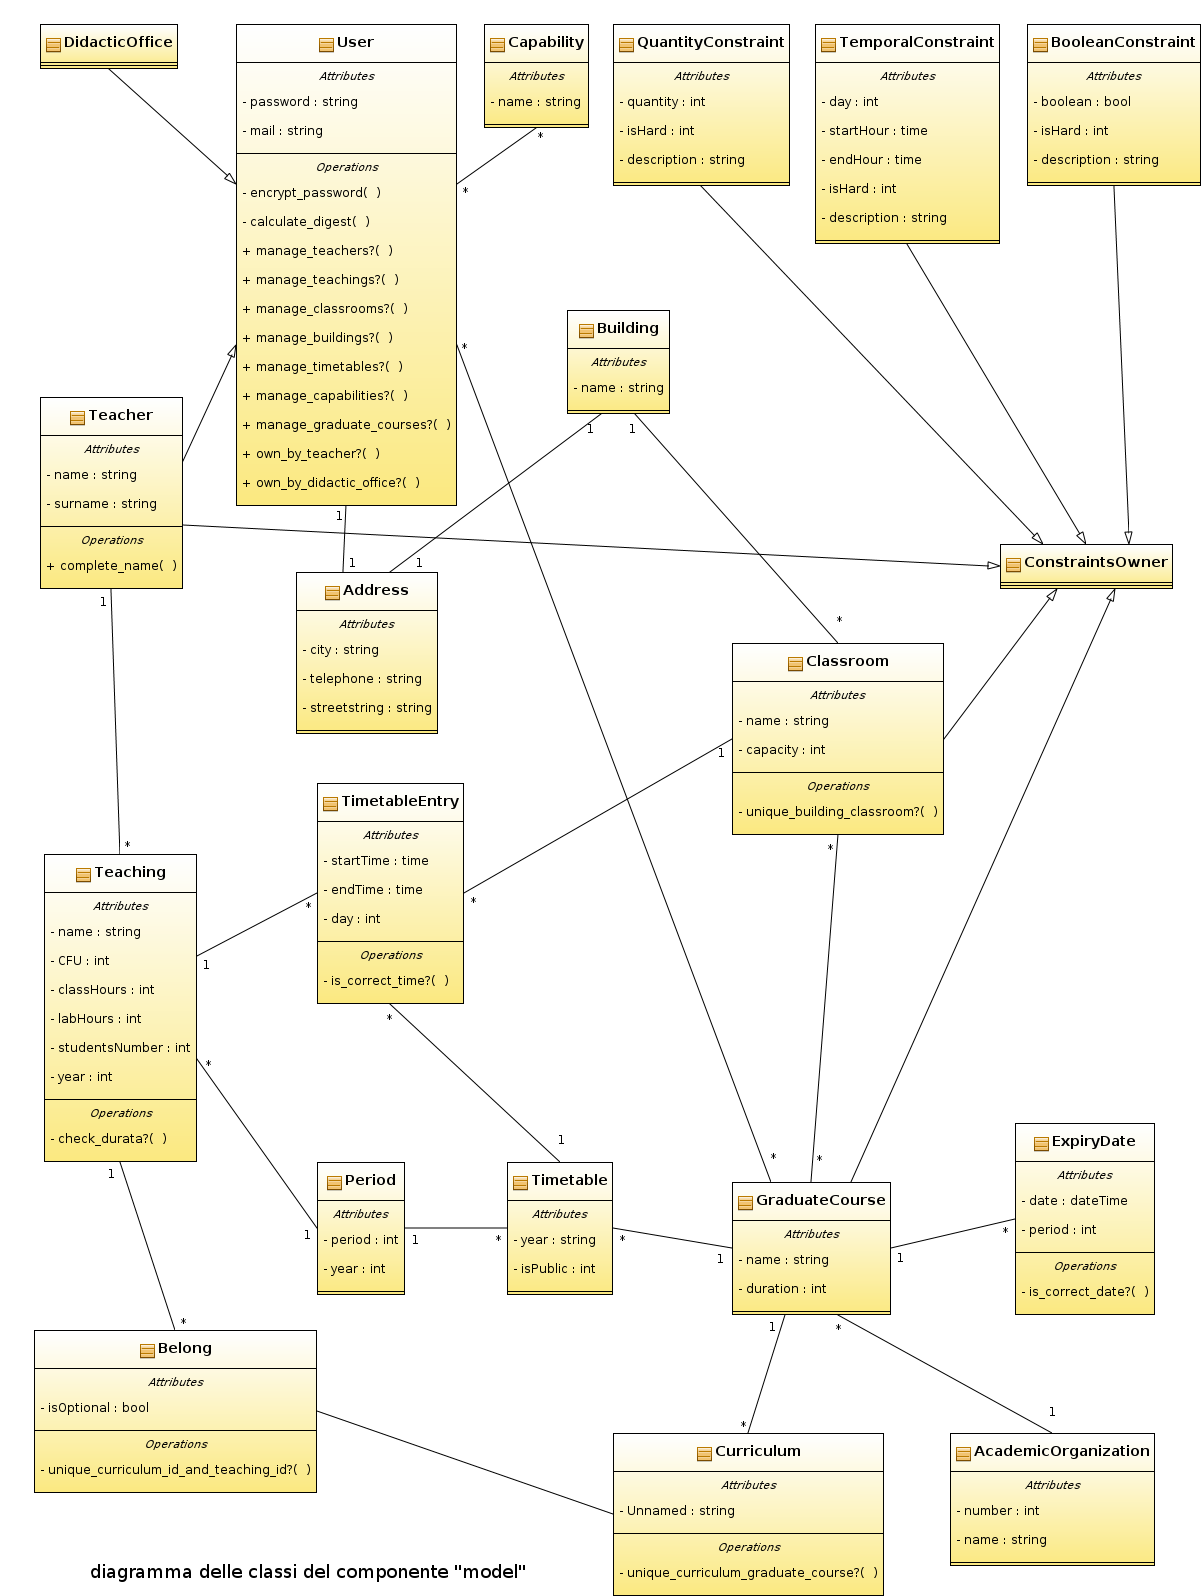
\includegraphics[scale=0.34]{images/Model_ClassDiagram.png}
\subsubsection{AcademicOrganization}
\subsubsection*{Descrizione degli attributi}
\begin{itemize}
 \item name: contiene il nome del tipo di organizzazione accademica; ad esempio Trimestre.
 \item number: contiene il numero di periodi dell'organizzazione accademica
\end{itemize}
\subsubsection*{Validazioni}
\begin{itemize}
 \item \verb|name|:\\ nella tabella \verb|academic_organizations| non deve essere presente una tupla con lo stesso valore dell'attributo. La stringa non dovrà essere nulla e dovrà essere al massimo di 30 caratteri. Infine dovrà rispettare la seguente espressione regolare: \verb|/^[a-zA-Zàòèéùì\s]*$/|
\item \verb|number|:\\ nella tabella \verb|academic_organizations| non deve essere presente una tupla con lo stesso valore contenuto nell'attributo. Inoltre potrà assumere solo valori interi compresi tra 1 e 6
\end{itemize}
\subsubsection*{Funzioni di callback}
\paragraph{before\_validation}
Prima di effettuare le operazioni di validazione, verrà reso maiscuolo il primo carattere del contenuto dell'attributo \verb|name| e minuscoli i rimanenti.
\subsubsection{Address}
\subsubsection*{Descrizione degli attributi}
\begin{itemize}
 \item street: contiene la via  
 \item city: contiene il nome della città
 \item telephone: contiene un numero di telefono
\end{itemize}
\subsubsection*{Validazioni}
Le validazioni di \verb|city| e di \verb|street| sono identiche all'attributo \verb|name| del model \verb|AcademicOrganization|
\begin{itemize}
 \item \verb|telephone|: il numero di telefono dovrà essere al massimo di 13 caratteri e dovrà rispettare l'espressione regolare\\
 \verb|/^[0-9]{2,4}-[0-9]{6,8}$/|.\\  
In questo modo il contenuto di \verb|telephone| avrà un numero di cifre compreso tra due e quattro(prefisso), seguite dal simbolo - ed infine un secondo numero di cifre compreso tra sei e otto (numero di telefono). Non è necessario inserire e controllare prima del numero di telefono il prefisso internazionale, perchè si ipotizza che tutti i numeri inseriti siano italiani.
\end{itemize}
\subsubsection*{Funzioni di callback}
\subsubsection*{before\_save}
Prima di salvare l'oggetto nel database, verrà reso maiuscolo il primo carattere del contenuto degli attributi \verb|city| e \verb|street| e minuscoli i rimanenti.
\subsubsection{Belong}
\subsubsection*{Descrizione degli attributi}
\begin{itemize}
 \item \verb|curriculum_id|: chiave esterna di curriculums
 \item \verb|teaching_id|: chiave esterna di teachings
 \item \verb|isOptional|: attributo booleano che indica se l'insegnamento individuato dalla chiave esterna \verb|teaching_id|, è opzionale rispetto al curriculum individuato della chiave esterna \verb|curriculum_id|	
\end{itemize}
\subsubsection*{Validazioni}
\begin{itemize}
 \item \verb|curriculum_id|: il contenuto della chiave esterna \verb|curriculum_id| non deve essere nullo 
 \item \verb|teaching_id|: il contenuto della chiave esterna \verb|teaching_id| non deve essere nullo
\end{itemize}
\subsubsection*{validate\_on\_create}
\begin{itemize}
 \item \verb|validate_on_create :unique_curriculum_id_and_teaching_id?|: \\E' possibile salvare nel database l'oggetto istanziato, solo se nessuna riga della tabella associata \verb|belongs|, ha gli stessi valori di \verb|teaching_id| e di \verb|curriculum_id| dell'istanza.\\
 \verb|unique_curriculum_id_and_teaching_id?| è un metodo privato utilizzato per la validazione precedente.
\end{itemize}
\subsubsection{Building}
\subsubsection*{Descrizione degli attributi}
\begin{itemize}
 \item \verb|name|: contiene il nome dell'edificio
 \item \verb|address_id|: chiave esterna di addresses	
\end{itemize}
\subsubsection*{Validazioni}
Le validazioni di \verb|name| sono identiche all'attributo \verb|name| del model \\ \verb|AcademicOrganization|
\begin{itemize}
 \item \verb|address_id|: il contenuto della chiave esterna non deve essere nullo
\end{itemize}
\subsubsection*{Funzioni di callback}
\subsubsection*{before\_validation}
Prima di effettuare le operazioni di validazione, verrà reso maiscuolo il primo carattere del contenuto dell'attributo \verb|name| e minuscoli i rimanenti.
\subsubsection{Capability}
\subsubsection*{Descrizione degli attributi}
\begin{itemize}
 \item \verb|name|: contiene il nome del privilegio disponibile per gli utenti del sistema
\end{itemize}
\subsubsection*{Validazioni}
Le validazioni di \verb|name| sono identiche all'attributo \verb|name| del model \\ \verb|AcademicOrganization|
\subsubsection{Classroom}
\subsubsection*{Descrizione degli attributi}
\begin{itemize}
 \item \verb|name|: contiene il nome dell' aula
 \item \verb|capacity|: contiene la capienza massima dell'aula
 \item \verb|building_id|: chiave esterna di \verb|buildings|	
\end{itemize}
\subsubsection*{Validazioni}
Le validazioni di \verb|name| sono identiche all'attributo \verb|name| del model \\ \verb|AcademicOrganization| senza il controllo dell'unicità.
\begin{itemize}
\item \verb|capacity|: il contenuto deve essere un intero compreso tra 0 e 1000. Sarà possibile lasciare questo attributo nullo.
\item \verb|building_id|: il contenuto della chiave esterna non deve essere vuoto 
\end{itemize}
\subsubsection*{Validate}
\begin{itemize}
 \item \verb|validate :unique_building_classroom?|: per salvare l'istanza nel database, è necessario che l'oggetto di tipo \verb|Building|, con chiave primaria uguale a \verb|building_id|, non abbia associato un oggetto di tipo \verb|Classroom| con \verb|name| uguale a quello definito nell'istanza.
\item \verb|unique_building_classroom?| è un metodo privato utilizzato nella validazione precedente
\end{itemize}
\subsubsection*{Funzioni di callback}
\subsubsection*{before\_validation}
Prima di effettuare le operazioni di validazione, verrà reso maiscuolo il primo carattere del contenuto dell'attributo \verb|name| e minuscoli i rimanenti.
\subsubsection{Curriculum}
\subsubsection*{Descrizione degli attributi}
\begin{itemize}
 \item \verb|name|: contiene il nome del curriculum
 \item \verb|graduate_course_id|: contiene la chiave esterna di \verb|graduate_courses|	 
\end{itemize}
\subsubsection*{Validazioni}
Le validazioni di \verb|name| sono identiche all'attributo \verb|name| del model \\ \verb|AcademicOrganization|, senza il controllo dell'unicità
\begin{itemize}
 \item \verb|graduate_course_id|: la chiave esterna di \verb|graduate_courses| non deve essere nulla
\end{itemize}
\subsubsection*{validate}
\begin{itemize}
 \item \verb|validate :unique_curriculum_graduate_course?|: per salvare l'oggetto nel database, è necessario che il graduate course, con id uguale a \verb|graduate_course_id|, non abbia associato un curriculum con il nome uguale a quello definito nell'oggetto
\item \verb|unique_curriculum_graduate_course?| è un metodo privato utilizzato nella validazione precedente.
\end{itemize}
\subsubsection*{Funzioni di callback}
\subsubsection*{before\_validation}
Prima di effettuare le operazioni di validazione, verrà reso maiscuolo il primo carattere del contenuto dell'attributo \verb|name| e minuscoli i rimanenti.
\subsubsection{ExpiryDate}
\subsubsection*{Descrizione degli attributi}
\begin{itemize}
 \item \verb|date|: successivamente a questa data, il docente non potrà più inserire le proprie indisponibilità
\end{itemize}
\subsubsection*{Validazioni}
\begin{itemize}
 \item \verb|date| : il contenuto di \verb|date| non deve essere vuoto
 \item \verb|graduate_course_id| : il contenuto della chiave esterna non deve essere vuoto
\end{itemize}
\subsubsection*{validate}
\begin{itemize}
 \item \verb|validate :is_correct_date?|: la data inserita deve essere maggiore della data di oggi. 
 \item \verb|is_correct_date?| è un metodo privato utilizzato nella validazione precedente
\end{itemize}

\subsubsection{GraduateCourse}
\subsubsection*{Descrizione degli Attributi}
\begin{itemize}
 \item \verb|name|: contiene il nome del corso di laurea
 \item \verb|duration|: indica la durata, in anni, del corso di laurea
\end{itemize}
\subsubsection*{Validazioni}
Le validazioni di \verb|name| sono identiche all'attributo \verb|name| del model \\ \verb|AcademicOrganization| eccezion fatta per il numero di caratteri di 50.
\begin{itemize}
\item \verb|:duration|: deve essere un intero compreso tra 1 e 6
\item \verb|academic_organization_id|: la chiave esterna non deve essere nulla. Quindi un oggetto di tipo \verb|GraduateCourse| per essere valido, deve avere associato un oggetto di tipo \verb|AcademicOrganization| anch'esso valido.
\end{itemize}
\subsubsection*{Funzioni di callback}
\subsubsection*{before\_validation}
Prima di effettuare le operazioni di validazione, verrà reso maiscuolo il primo carattere del contenuto dell'attributo \verb|name| e minuscoli i rimanenti.
\subsubsection{Period}
\subsubsection*{Descrizione degli attributi}
\begin{itemize}
 \item \verb|subperiod|: individua un determinato periodo dell'anno accademico. Ad esempio in un corso di laurea con un'organizazzione a trimestri, \verb|subperiod| con valore 1 identifica il primo trimestre
 \item \verb|year|: individua l'anno, insteso come primo, secondo, terzo, ecc.
\end{itemize}
\subsubsection*{Validazioni}
\begin{itemize}
 \item \verb|subperiod|: dovrà contenere un valore intero compreso tra 1 e 4
\item \verb|year|: dovrà contenere un valore intero compreso tra 1 e 6
\end{itemize}
\subsubsection*{validate\_on\_create} 
\begin{itemize}
 \item \verb|validate_con_create :unique_subperiod_year?|: l'oggetto è valido solo se nella tabella \verb|periods| non è presente nessuna riga con gli stessi valori di \verb|period| e di \verb|year| dell'istanza.
 \item \verb|unique_subperiod_year?| è un metodo privato utilizzato nella validazione precedente
\end{itemize}
\subsubsection{Teacher}
\subsubsection*{Descrizione degli attributi}
\begin{itemize}
 \item \verb|name|: contiene il nome del docente
 \item \verb|surname|: contiene il cognome del docente
\end{itemize}
\subsubsection*{Validazioni}
Le validazioni di \verb|name| e di \verb|surname| sono identiche all'attributo \verb|name| del model \verb|AcademicOrganization|. Non è presente però la validazione di unicità. In questo modo sono ammessi i casi di omonimia.
\subsubsection*{Funzioni di callback}
\subsubsection*{before\_validation}
Prima di effettuare le operazioni di validazione, verrà reso maiscuolo il primo carattere del contenuto degli attributi \verb|name| e \verb|surname| e minuscoli i rimanenti.
\subsubsection*{before\_destroy}
Prima di eliminare l'oggetto verrà eliminato lo user ad esso associato.
\subsubsection{Teaching}
\subsubsection*{Descrizione degli attributi}
\begin{itemize}
 \item \verb|name|: contiene il nome dell'insegnamento
 \item \verb|CFU|: contiene il numero di crediti formativi dell'insegnamento
 \item \verb|classHours|: contiene il numero di ore settimanali di lezione in aula
 \item \verb|labHours|: contiene il numero di ore settimanali di lezione in laboratorio
 \item \verb|studentsNumber|: contiene la stima del numero di studenti che frequenteranno l'insegnamento 
\end{itemize}
\subsubsection*{Validazioni}
Le validazioni di \verb|name| sono identiche all'attributo \verb|name| del model \\ \verb|AcademicOrganization|. Inoltre è permesso l'inserimento nella stringa di valori numerici.
\begin{itemize}
 \item \verb|CFU|: per essere valido deve contenere un valore intero compreso tra 1 e 20
 \item \verb|labHours, classHours|: gli attributi per essere validi devono contenere un valore intero compreso tra 0 e 50
\item \verb|studentsNumber|: per essere valido deve contenere un valore intero compreso tra 1 e 1000
\end{itemize}
Tutti questi attributi possono essere nulli. Questo perchè non si può sempre sapere all'atto della creazione dell'insegnamento, il numero di ore di lezione o la stima del numero di studenti che frequenteranno il corso d'insegnamento.
\begin{itemize}
 \item \verb|period_id|: la chiave esterna non deve essere nulla. Questo significa che l'oggetto istanziato deve essere associato ad un periodo valido.
\end{itemize}
\subsubsection*{validate}
\begin{itemize}
\item \verb|validate :check_durata?|: un insegnamento può appartenere a più curriculum; due diversi curriculum possono avere un insegnamento in comune, ma appartenere a due differenti corsi di laurea con diversa organizzazione accademica.
Per questo motivo un \verb|Teaching| è valido solo se l'oggetto \verb|Period| associato, ha un valore di \verb|year| minore o uguale al minimo valore dell'attributo \verb|duration| scelto fra tutti i \verb|GraduateCourse|, che hanno almeno un \verb|Curriculum| associato a quel \verb|Teaching|. Ovviamente dovrà essere confrontato anche l'attributo \verb|subperiod| (appartenente al model \verb|Period| associato) con l'attributo \verb|number|.
\item \verb|check_durata?| è un metodo privato utilizzato nella precedente validazione.
\end{itemize}
\subsubsection*{Funzioni di callback}
\subsubsection*{before\_validation}
Prima di effettuare le operazioni di validazione, verrà reso maiscuolo il primo carattere del contenuto dell'attributo \verb|name|.
\subsubsection{TimeTable}
\paragraph{Descrizione degli attributi}
 \begin{itemize}
  \item \verb|year|: contiene l'anno accademico. Ad esempio 2008-09
  \item \verb|period_id|: chiave esterna di \verb|periods|
  \item \verb|graduate_course_id|: chiave esterna di \verb|graduate_courses|
 \end{itemize}
\subsubsection*{Validazioni}
\subsubsection*{Attributi year,period\_id,graduate\_course\_id}
\begin{itemize}
 \item \verb|year, period_id, graduate_course_id|: il contenuto degli attributi devono essere non nulli.
 \item \verb|year| : deve rispettare l'espressione regolare\\ \verb|/^[0-9]{4,4}-[0-9]{2,2}$/|; dovrà avere nei primi quattro caratteri solo cifre, il quinto dovrà essere riservato al carattere - ed infine negli ultimi due caratteri dovranno esserci altri due numeri
\end{itemize}
\subsubsection{TimetableEntry}
\subsubsection*{Descrizione degli attributi}
\begin{itemize}
 \item \verb|startTime|: contiene un oggetto di tipo Time e indica l'ora di inizio
 \item \verb|endTime|: contiene un oggetto di tipo Time e indica l'ora di fine
 \item \verb|day|: contiene un intero che indica un determinato giorno della settimana.
 \item \verb|teaching_id|: chiave esterna di \verb|teachings|
 \item \verb|classroom_id|: chiave esterna di \verb|classrooms|
 \item \verb|timetable_id|: chiave esterna di \verb|timetables|
\end{itemize}
\verb|startTime|,\verb|endTime| e \verb|day|\\ individuano quando verrà svolta la lezione del corso d'insegnamento, individuato dalla chiave esterna \verb|teaching_id|. \verb|classroom_id| individuerà l'aula che verrà utilizzata.
\subsubsection*{Validazioni}
\begin{itemize}
 \item \verb|startTime, endTime, day | \verb|timetable_id, classroom_id|: Nessun attributo dell'oggetto deve essere nullo.
 \item \verb|:day|: deve essere un intero compreso tra 1 e 6
\end{itemize}
\subsubsection*{validate}
\begin{itemize}
\item \verb|validate :is_correct_time?|: L'oggetto d'istanza è valido solo se l'attributo \verb|startTime| ha un oggetto di tipo tempo minore dell'oggetto contenuto in \verb|endTime|.
\item \verb|:is_correct_time?| è un metodo privato usato le validazione precedente
\end{itemize}
\subsubsection{User}
\subsubsection*{Descrizione degli attributi}
\begin{itemize}
 \item \verb|mail|: contiene una stringa che rappresenta la mail dello user
 \item \verb|password|: contiene la password(crittografata tramite SHA1) dello user
 \item \verb|random|: contiene un valore casuale, che verrà utilizzato per calcolare il digest.
 \item \verb|digest|: il contenuto dell'attributo \verb|mail| concatenato al valore di \verb|random|, viene crittografato tramite SHA1. Il risultato dell'operazione verrà salvato in questo attributo.
\end{itemize}
\subsubsection*{Validazioni}
\begin{itemize}
\item \verb|password, mail, random, digest|: tutti gli attributi devono essere non nulli. Per \verb|password| il controllo della presenza di contenuto non nullo, verrà eseguito solo nelle operazioni di aggiornamento e non nelle operazioni di creazione. Questo perchè un utente verrà inizialmente inserito nel sistema e successivamente verrà invitato tramite mail a completare la registrazione inserendo la password. 
\item \verb|password|: dovrà contenere come minimo 6 caratteri e dovrà rispettare l'espressione regolare: \verb|/^[a-zA-Z0-9\.]*$/|. 
 \item \verb|mail|: nella tabella \verb|users| non deve essere presente una tupla con lo stesso valore dell'attributo \verb|mail| dell'oggetto istanziato. Non possono esistere due user con lo stesso indirizzo e-mail. Inoltre il contenuto deve rispettare l'espressione regolare:\\
\verb|^([a-zA-Z0-9_\.\-\+]){4,20}\@|\\ \verb|(([a-zA-Z0-9\-])+\.)+([a-zA-Z0-9]{2,4})$/|.\\
Si accettano tutti i tipi di indirizzo e-mail con un numero di caratteri compreso tra 4 e 20. E' possibile utilizzare lettere maiuscole, minuscole, numeri e i caratteri - e +. Sono valide anche le mail che hanno più domini, come ad esempio prova@math.unipd.it 
\end{itemize}
\subsubsection*{Funzioni di callback}
\begin{itemize}
 \item \verb|before_save :encrypt_password|: prima di salvare l'oggetto di tipo \verb|User| nel database, la password viene crittografata attraverso l'algoritmo SHA1. 
\item \verb|encrypt_password| è un metodo privato. utilizzato nella precedente funzione.
\item \verb|before_validation :calculate_digest|: prima di validare l'oggetto, viene chiamato il metodo \verb|calculate_digest|. Questo metodo calcola il digest, tramite l'algoritmo SHA1, della stringa contenuta in \verb|mail|, concatenata ad un numero casuale (contenuto nell'attributo \verb|random|). Il risultato infine viene salvato nell'attributo \verb|digest|. 
\item \verb|calculate_digest| è un metodo privato utilizzato nella precedente funzione.
\end{itemize}
\paragraph{Metodi pubblici}
Nel model \verb|User| sono presenti diversi metodi pubblici che ritornano true se l'oggetto possiede uno specifico privilegio. Ogni metodo inizierà con la radice \verb|manage_|:
\begin{itemize}
 \item \verb|manage_teachers?|: ritorna true se l'utente possiede il privilegio di amministrazione dei docenti
 \item \verb|manage_teachings?|: ritorna true se l'utente possiede il privilegio di amministrazione degli insegnamenti
 \item \verb|manage_classrooms?|: ritorna true se l'utente possiede il privilegio di amministrazione delle aule
 \end{itemize}
Non è necessario riportare tutti i metodi, dato che il loro scopo è facilmente intuibile dalla denominazione;

I metodi \verb|own_by_teacher?| e \verb|own_by_didactic_office?|, indicano se l'oggetto appartiene ad un \verb|Teacher| o ad un \verb|DidacticOffice|.
\subsubsection{DidacticOffice}
\subsubsection*{Funzioni di callback}
\begin{itemize}
 \item \verb|before_destroy|: prima dell'eliminazione di un oggetto di tipo \\ \verb|DidacticOffice|, viene eliminato l'oggetto di tipo \verb|User| ad esso associato.
\end{itemize}
\subsubsection{TemporalConstraint}
\subsubsection*{Descrizione degli attributi}
\begin{itemize}
 \item \verb|startHour|:contiene un oggetto di tipo \verb|Time| ed indica l'ora di inizio dell'indisponibilità
 \item \verb|endHour|: contiene un oggetto di tipo \verb|Time| ed indica l'ora di fine dell'indisponibilità
 \item \verb|day|: contiene un intero che individua il giorno dell'indisponibilità
\end{itemize}
\subsubsection*{Validazioni}
\begin{itemize}
 \item \verb|startHour,endHour,day|: tutti gli attributi devono essere non nulli
 \item \verb|day|: deve contenere un valore intero compreso tra 1 e 6
 \end{itemize}
\subsubsection*{validate}
\begin{itemize}
 \item \verb|validate :is_correct_time?|: l'oggetto è valido solo se \verb|starthour| è minore di \verb|endHour|. \item \verb|is_correct_time?| è un metodo privato utilizzato nella precedente validazione.
\end{itemize}
\subsubsection{QuantityConstraint}
\subsubsection*{Descrizione degli attributi}
\begin{itemize}
 \item \verb|quantity|: contiene un valore intero rappresentante la quantità del vincolo o preferenza
\end{itemize}
\subsubsection*{Validazioni}
\begin{itemize}
 \item \verb|quantity|: il contenuto di \verb|quantity| deve essere presente
 \item \verb|validates_numericality_of :quantity|: il contenuto di \verb|quantity| deve essere un intero compreso tra 1 e 1000 
\end{itemize}
\subsubsection{BooleanConstraint}
\subsubsection*{Descrizione attributi}
\begin{itemize}
 \item \verb|bool|: contiene un valore booleano rappresentante la presenza o meno del vincolo o preferenza
\end{itemize}
\subsubsection*{Validazioni}
\begin{itemize}
 \item \verb|bool|: il contenuto di \verb|bool| deve essere presente
\end{itemize}
I model \verb|BooleanConstraint|, \verb|TemporalConstraint| e \verb|QuantityConstraint|
hanno in comune i seguenti attributi:
\begin{itemize}
 \item \verb|description|: contiene una descrizione del vincolo
 \item \verb|isHard|: contiene un valore di tipo intero. Se questo è uguale a 0, significa che rappresenta un vincolo, mentre un valore maggiore o uguale ad 1 indica una preferenza con importanza inversamente proporzionale al numero.
 \end{itemize}
\subsubsection{ConstraintsOwner}
All'interno di questa classe, si definiranno le relazioni tra i vincoli e i relativi proprietari.
Un vincolo può avere come proprietario: un corso di laurea (\verb|GraduateCourse|), una classe (\verb|Classroom|) o un docente (\verb|Teacher|).
Un proprietario, può avere tre tipi di vincoli, booleano, temporale e di quantità.
Grazie a questo model join ed al plugin \verb|has_many_polymorphs|, sarà possibile associare in modo semplice e veloce un proprietario con un qualsiasi tipo di vincolo
\subsubsection{TeacherMailer}
La classe \verb|TeacherMailer| che si occupa dell'invio delle e-mail per l'attivazione dell'account del docente può essere considerata, in modo astratt, appartene alla componente Model. Essa deriva dalla classe \verb|ActionMailer::Base| presente nel framework Rails ed implementa il metodo \verb|activate_teacher(sender, receiver)| che si occupa dell'invio del link per l'attivazione dell'account del docente.
\subsection{Database}
L'integrità referenziale è un concetto molto importante da non dimenticare durante la progettazione di un database.
Da poco MySql ha implementato un supporto per la chiavi esterne attraverso il nuovo table engine INNODB.

La sintassi per aggiungere un vincolo d'integrità alle chiave esterne è il seguente:\\
\verb|add constraint constraint_name| \\
\verb|foreign key (from_column)|\\
\verb|references to_table(id)|\\
Ovviamente ogni tabella del database dovrà utilizzare come engine INNODB, altrimenti la clausula \verb|foreign key| verrà ignorata.
\subsection{Componente Controller}
La componente Controller si occupa di gestire le azioni che l'utente effettua, solitamente attraverso una view. Ogni metodo pubblico rappresenta quindi una specifica azione, eccezion fatta per l'Application Controller.
Di seguito è riportato il diagramma delle classi che illustra questa componente. Sono stati omessi volutamente i tipi di ritorno per i metodi che implementano un'azione, in quanto queste operazioni non sono utilizzate per restituire un valore, bensì inizializzano alcune variabili d'istanza che saranno successivamente disponibili nella view specifica per quella azione. Inoltre per aumentare la leggibilità è stata omessa la derivazione della classe \verb|ApplicationController| da \verb|ActionController::Base|. \\
\bigskip \\
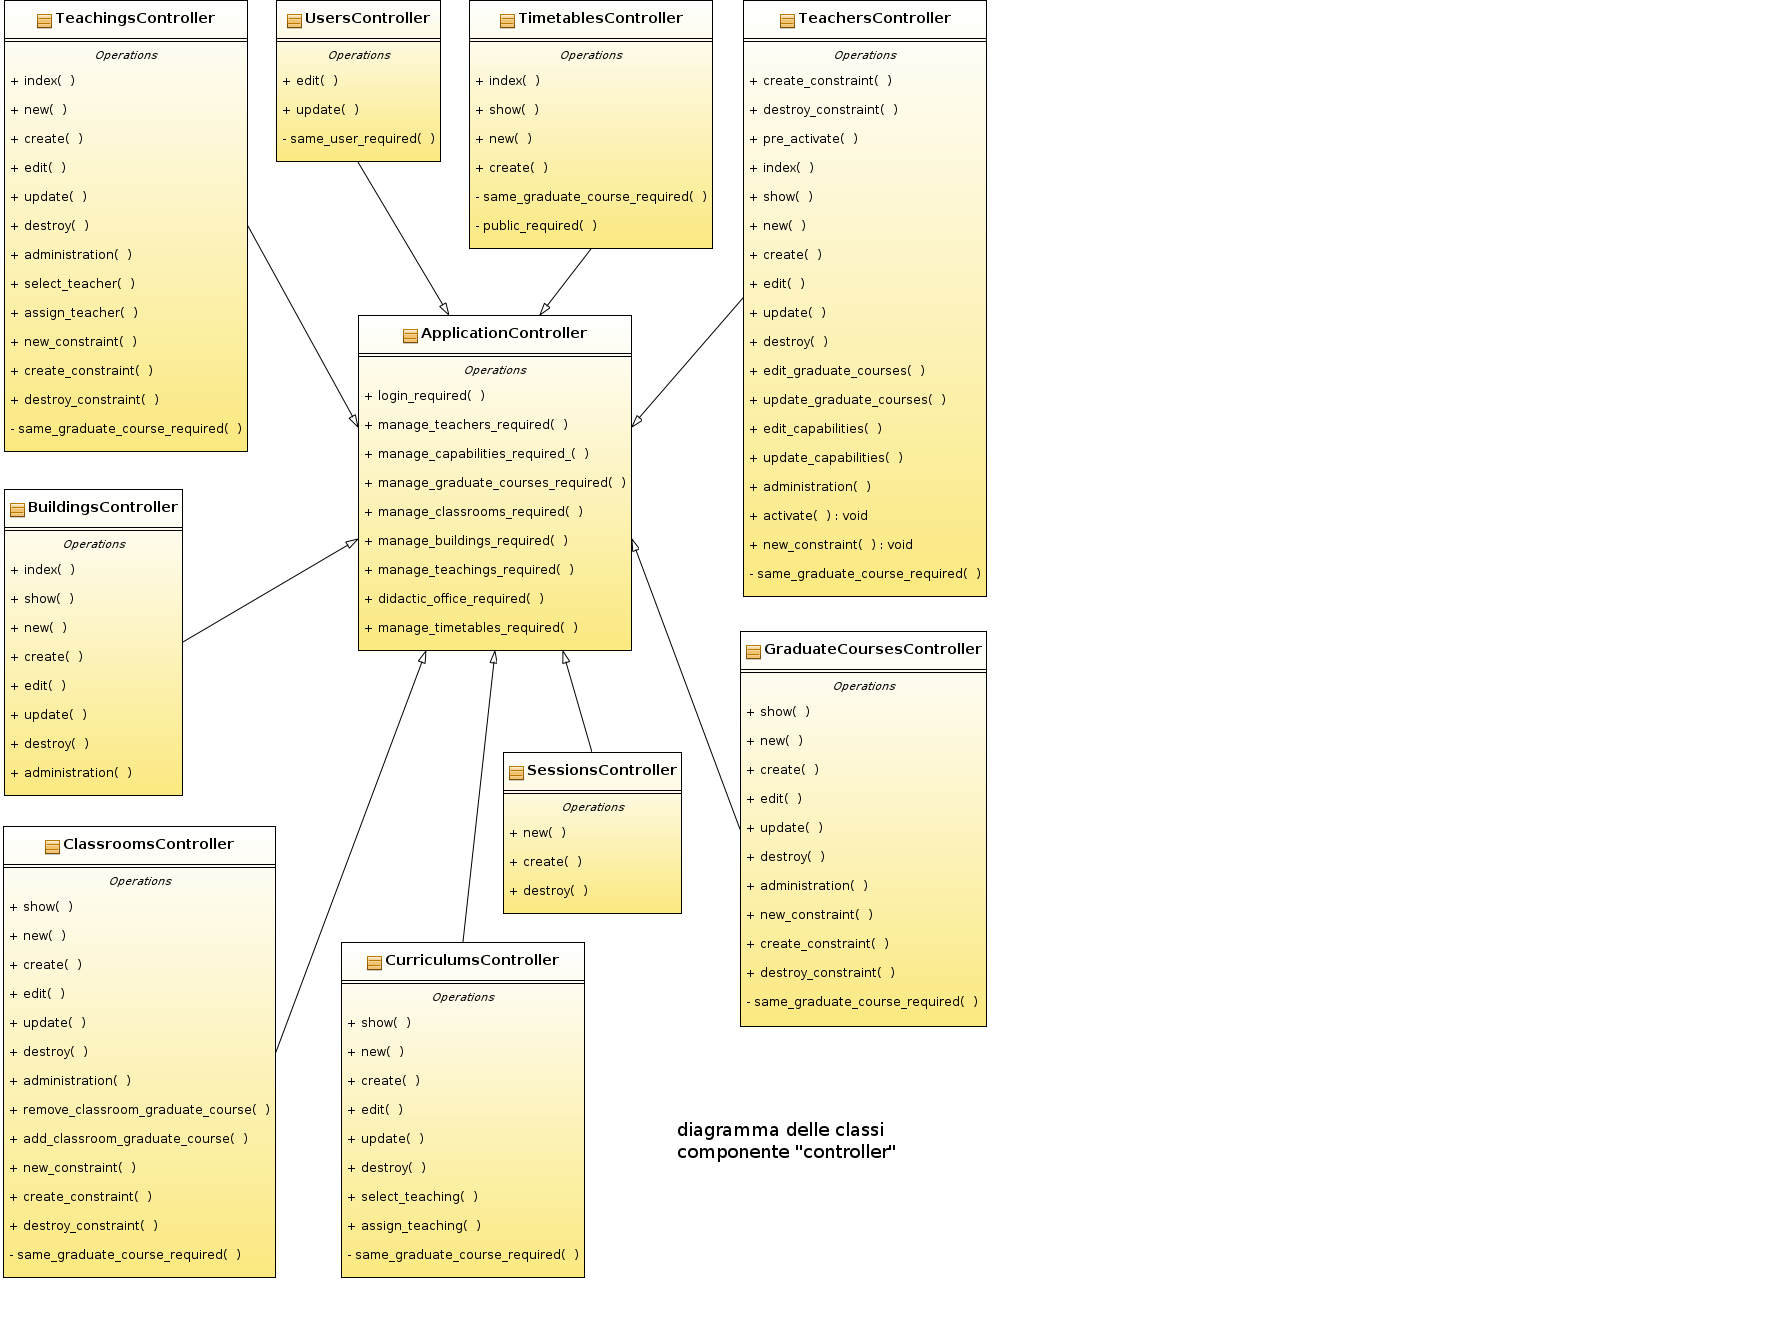
\includegraphics[scale=0.34]{images/Controller_ClassDiagram.png}
\subsubsection{Azioni comuni a più controller}
Per evitare fastidiose ripetizioni in questa sezione verranno descritti i metodi che figurano con lo stesso nome in diversi controller. La scelta dello stesso nome non è casuale, in quanto rispecchia la funzione dell'azione.
\begin{itemize}
 \item \verb|index|: rende disponibile alla view specifica un insieme d'istanze ed è raggiungibile eseguendo una richiesta GET all'indirizzo /nomecontroller. Ad esempio l'azione \verb|index| di \verb|GraduateCourseController| fornisce alla view un insieme di corsi di laurea ed è raggiungibile attraverso una richiesta GET all'indirizzo /graduate\_courses.
 \item \verb|show|: rende disponibile alla view specifica un'istanza ed è raggiungibile eseguendo una richiesta GET all'indirizzo /nomecontroller/id. Usando sempre l'esempio dei corsi di laurea, eseguendo una richiesta GET all'indirizzo /graduate\_courses/1 verranno visualizzate le informazioni relative al corso di laurea con id 1.
 \item \verb|new|: rende disponibile alla view specifica un'istanza vuota per permettere l'inserimento di un nuovo oggetto. E' raggiungibile eseguendo una richiesta GET /nomecontroller/new
 \item \verb|create|: acquisisce i dati da una richiesta POST per salvare l'oggetto nel database attraverso il model. Solitamente i dati provengono da una form con metodo POST presente nella view per l'azione \verb|new|. E' possibile comunque invocare questa azione mediante una richiesta POST all'indirizzo /nomecontroller
 \item \verb|edit|: rende disponibile alla view specifica un'istanza esistente per permetterne la modifica. e' raggiungibile attraverso una richiesta GET all'indirizzo /nomecontroller/id/edit
 \item \verb|update|: acquisisce i dati da una richiesta PUT per aggiornare lo stato dell'oggetto nel database attraverso il model. Solitamente i dati provengono da una form con metodo PUT presente nella view per l'azione \verb|edit|. E' possibile comunque invocare questa azione mediante una richiesta PUT all'indirizzo /nomecontroller/id
 \item \verb|destroy|: distrugge l'oggetto attraverso il model. Questa azione viene invocata tramite una richiesta DELETE all'indirizzo /nomecontroller/id
 \item \verb|administration|: rende disponibile alla view specifica un insieme d'istanze per effettuarne l'amministrazione. Questa azione è raggiungibile attraverso una richiesta GET all'indirizzo \\ /nomecontroller/administration.
 \item \verb|new_constraint|: rende disponibile alla view specifica un'istanza per un vincolo od una preferenza per permetterne l'inserimento. E' raggiungibile eseguendo una richiesta GET all'indirizzo \\ /nomecontroller/id/new\_constraint
 \item \verb|create_constraint|: acquisisce i dati da una richiesta POST per salvare il vincolo o la preferenza nel database attraverso il model. Solitamente i dati provengono da una form con metodo POST presente nella view per l'azione \verb|new_constraint|. E' possibile comunque invocare questa azione mediante una richiesta POST all'indirizzo /nomecontroller/id/create\_constraint
 \item \verb|destroy_constraint|: distrugge l'oggetto attraverso il model. Questa azione viene invocata tramite una richiesta DELETE all'indirizzo /nomecontroller/id/destroy\_contraint/id
\end{itemize}
Solitamente non è necessaria l'autenticazione o il possesso di alcuni privilegi per eseguire le azioni \verb|index| e \verb|show|. Per quanto riguarda gli altri metodi, invece, può ritenersi necessaria l'autenticazione od il possesso di alcuni privilegi. Per ogni controller sarà descritto questo aspetto.
Differente invece è il caso del metodo \verb|same_graduate_course_required|, dichiarato privato nei controllers che lo implementano. Questo metodo non rispecchia un'azione, ma è utilizzato come filtro, ovvero è chiamato prima o dopo una determinata azione, per impedire la modifica o la cancellazione di un oggetto appartenente ad un corso di laurea diverso da quello dell'utente autenticato.
\subsubsection{ApplicationController}
Questa classe deriva direttamente da \verb|ActionController::Base|, ed è estesa da ogni controller. Prevede metodi di pubblica utilità per gli altri controller, ma nessuna azione. L' \verb|ApplicationController| del sistema Sigeol prevede i seguenti metodi pubblici, utilizzati come filtri dagli altri controller.
\begin{itemize}
 \item \verb|login_required|: se l'utente non è autenticato questo metodo reindirizza alla pagina di login
 \item \verb|manage_teachers_required|: se l'utente non possiede i privilegi per gestire i docenti questo metodo reindirizza alla pagina principale mostrando un errore.
 \item \verb|manage_capabilities_required|: se l'utente non possiede i privilegi per gestire i privilegi questo metodo reindirizza alla pagina principale mostrando un errore.
 \item \verb|manage_graduate_courses_required|: se l'utente non possiede i privilegi per gestire i corsi di laurea questo metodo reindirizza alla pagina principale mostrando un errore.
 \item \verb|manage_classrooms_required|: se l'utente non possiede i privilegi per gestire le aule questo metodo reindirizza alla pagina principale mostrando un errore.
 \item \verb|manage_buildings_required|: se l'utente non possiede i privilegi per gestire gli edifici questo metodo reindirizza alla pagina principale mostrando un errore.
 \item \verb|manage_teachings_required|: se l'utente non possiede i privilegi per gestire gli insegnamenti questo metodo reindirizza alla pagina principale mostrando un errore.
 \item \verb|manage_timetables_required|: se l'utente non possiede i privilegi per gestire gli orari questo metodo reindirizza alla pagina principale mostrando un errore.
 \item \verb|didactic_office_required|: se l'utente non appartiene ad una segreteria didattica questo metodo reindirizza alla pagina principale mostrando un errore.
\end{itemize}
\subsubsection{GraduateCoursesController}
Il controller \verb|GraduateCourseController| permette alla segreteria didattica di creare e eliminare i corsi di laurea. Inoltre permette agli utenti con gli opportuni privilegi di aggiornare le informazioni relative ai propri corsi di laurea.
I filtri utilizzati in questo controller vengono tutti anteposti alle azioni e sono i seguenti:
\begin{itemize}
 \item \verb|login_required| non è utilizzato nelle azioni \verb|index| e \verb|show|
 \item \verb|manage_graduate_courses_required| è utilizzato nelle azioni \verb|edit|, \verb|update|, \verb|destroy|, \verb|administration|
 \item \verb|didactic_office_required| è utilizzato nelle azioni \verb|new|, \verb|create| e \verb|destroy|
 \item \verb|same_graduate_course_required| è utilizzato nelle azioni \verb|edit|,\\ \verb|update|, e \verb|destroy|.
\end{itemize}
\subsubsection{CurriculumsController}
Il controller \verb|CurriculumsController| permette all'utente con gli opportuni privilegi di creare, modificare ed eliminare le informazioni relative ai curricula dei propri corsi di laurea, nonchè di aggiungere o rimuove insegnamenti da quest'ultimi attreverso i metodi \verb|select_teaching|, raggiungibile medianta una richiesta GET all'indirizzo /curriculums/id/select\_teaching, e \verb|assign_teaching|, raggiungibile mediante una richiesta POST all'indirizzo /curriculums/id/assign\_teaching. Il primo fornisce alla view una lista degli insegnamenti presenti nel corso di laurea a cui il curriculum appartiene, mentre il secondo crea questa associazione tramite il model.
I filtri utilizzati in questo controller vengono tutti anteposti alle azioni e sono i seguenti:
\begin{itemize}
 \item \verb|login_required| non è utilizzato solamente nell'azione \verb|show|
 \item \verb|manage_graduate_courses_required| non è utilizzato solamente nell'azione \verb|show|
 \item \verb|same_graduate_course_required| è utilizzato nelle azioni \verb|edit|,\\ \verb|update|, \verb|select_teaching| e \verb|assign_teaching|.
\end{itemize}
\subsubsection{UsersController}
Il controller \verb|UsersController| dispone solamente delle azioni \verb|edit| e \verb|update| e del metodo privato \verb|same_user_required| (utilizzato come filtro anteposto alle due azioni assieme al filtro \verb|login_required|). Questa scelta progettuale deriva dalla relazione tra i model \verb|Teacher|, \verb|DidacticOffice| e \verb|User|. Confrontare la sezione \ref{model}.
Il metodo privato \verb|same_user_required| garantisce che non si stia cercando di modificare un utente diverso dal proprio.
\subsubsection{TeachersController}
Il controller \verb|TeachersController| permette all'utente con gli opportuni privilegi di creare, modificare ed eliminare i docenti dei propri corsi da laurea, nonchè di attribuire ad essi nuovi privilegi e corsi di laurea. Attraverso l'azione \verb|new| viene rischiesto un indirizzo e-mail di un docente e l'azione \verb|create| verificherà se questo è presente o meno nel database. Nel primo caso se il docente appartiene già a quel corso di laurea verrà segnalato un errore, altrimenti verrà aggiunto; nel secondo caso verrà inviata al nuovo docente una mail con le istruzioni per la registrazione al sistema. Il nuovo docente tramite l'azione \verb|pre_activate|, raggiungibile mediante una richista GET all'indirizzo /teachers/id/pre\_activate?digest=, potrà completare la creazione dello proprio user, e del relativo indirizzo, che sarà delegata all'azione \verb|activate|, raggiungibile mediante una richiesta POST all'indirizzo /teachers/id/activate?digest=. La certezza che solamente il docente invitato potrà creare il proprio account è resa possibile tramite il parametro \verb|digest| che solamente chi ha ha ricevuto la mail di invito può conoscere.

Infine attraverso le azioni \verb|edit_graduate_courses|, \verb|edit_capabilities|, \verb|update_graduate_courses| e \verb|update_capabilities|, raggiungibili rispettivamente mediante una richiesta GET all'indirizzo \\ /teachers/id/edit\_graduate\_courses o /teachers/id/edit\_capabilities e mediante una richiesta POST all'indirizzo /teachers/is/update\_graduate\_courses o /teachers/id/update\_capabilities, è possibilile modificare o rimuovere corsi di laurea e privilegi ai docenti da user che ne hanno la facoltà.
I filtri utilizzati in questo controller vengono tutti anteposti alle azioni e sono i seguenti:
\begin{itemize}
 \item \verb|login_required| non è utilizzato nelle azioni \verb|index|, \verb|show| ed \verb|activate|
 \item \verb|manage_teachers_required|  è utilizzato nelle azioni \verb|new|, \verb|create|,\\ \verb|administration|, \verb|edit_graduate_courses|, \verb|update_graduate_courses|
 \item \verb|manage_capabilities_required| è utilizzato nelle azioni \\ \verb|edit_capabilities| e \verb|update_capabilities|
 \item \verb|same_graduate_course_required| è utilizzato nelle azioni \\ \verb|edit_graduate_courses|, \verb|edit_capabilities|,\\ \verb|update_graduate_courses| e \verb|update_capabilities|.
\end{itemize}
\subsubsection{SessionsController}
Il controller \verb|SessionsController| permette la creazione di una sessione al momento dell'autenticazione dello user. Utilizza quindi le azioni \verb|new|, \verb|create| e \verb|destroy| senza alcun filtro, raggiungibili rispettivamente con una richiesta GET all'indirizzo /session/new, POST all'indirizzo /session e DELETE all'indirizzo /session/id.
\subsubsection{TeachingsController}
Il controller \verb|TeachingsController| permette all'utente con gli opportuni privilegi di creare, modificare ed eliminare le informazioni relative agli insegnamenti dei propri corsi di laurea, nonchè di aggiungere o rimuove il docente che tiene l'insegnamento in questione attraverso le azioni \verb|select_teacher|, raggiungibile medianta una richiesta GET all'indirizzo \\ /teachings/id/select\_teacher, e \verb|assign_teacher|, raggiungibile mediante una richiesta POST all'indirizzo /teachers/id/assign\_teacher. Il primo fornisce alla view una lista dei docenti presenti nel corso di laurea a cui il curriculum appartiene, mentre il secondo crea questa associazione tramite il model.
I filtri utilizzati in questo controller vengono tutti anteposti alle azioni e sono i seguenti:
\begin{itemize}
 \item \verb|login_required| non è utilizzato nelle azioni \verb|index| e \verb|show|
 \item \verb|manage_teachings_required| non è utilizzato nelle azioni \verb|index| e \verb|show|
 \item \verb|same_graduate_course_required| è utilizzato nelle azioni \verb|edit|,\\ \verb|update|, \verb|destroy|, \verb|select_teacher| e \verb|assign_teacher|.
\end{itemize}
\subsubsection{BuildingsController}
Il controller \verb|BuildingsController| permette all'utente con gli opportuni privilegi di creare, modificare ed eliminare le informazioni relative agli edifici ed ai relativi indirizzi.
I filtri utilizzati in questo controller vengono tutti anteposti alle azioni e sono i seguenti:
\begin{itemize}
 \item \verb|login_required| non è utilizzato nelle azioni \verb|index| e \verb|show|
 \item \verb|manage_buildings_required| non è utilizzato nelle azioni \verb|index| e \verb|show|
\end{itemize}
Non è presente il filtro \verb|same_graduate_course_required| in quanto un edificio non appartiene ad uno o più corsi di laurea, bensì all'intero sistema universitario.
\subsubsection{ClassroomsController}
Il controller \verb|ClassroomsController| permette all'utente con gli opportuni privilegi di creare, modificare ed eliminare le informazioni relative alle aule, nonchè di aggiungere o rimuovere le aule ai propri corsi di laurea attraverso le azione \verb|add_classroom_graduate_course| e \\ \verb|remove_classroom_graduate_course| raggiungibili attraverso una richiesta POST agli indirizzi, rispettivamente,\\ /classrooms/id/add\_classroom\_graduate\_course e \\ /classrooms/id/remove\_classroom\_graduate\_course
I filtri utilizzati in questo controller vengono tutti anteposti alle azioni e sono i seguenti:
\begin{itemize}
 \item \verb|login_required| non è utilizzato solamente nell'azione \verb|show|
 \item \verb|manage_classrooms_required| non è utilizzato solamente nell' azione \verb|show|
 \item \verb|same_graduate_course_required| non è utilizzato nelle azioni \verb|show|, \verb|new| e \verb|create|
\end{itemize}
\subsubsection{TimetablesController}
Il controller \verb|TimetablesController| permette all'utente con gli opportuni privilegi di creare ed eliminare gli orari.
Implementa alcune azioni aggiuntive oltre a quelle di base:
\begin{itemize}
\item \verb|schedule|: metodo usato nella creazione di una nuova istanza di schedulazione. Invia al MiddleMan (attraverso richiesta HTTP) i dati necessari ad impostare una nuova schedulazione.
\item \verb|notify|: metodo richiamato (attraverso richiesta HTTP) dal componente MiddleMan per notificare all'applicazione l'attivazione di un'evento precedentemente schedulato. Inoltre richiama il metodo \verb|start| per avviare la generazione dell'orario.
\item \verb|done|: metodo richiamato (attraverso richiesta HTTP) dal componente MiddleMan utilizzato per segnalare la fine del calcolo.
\item \verb|start|: metodo che segnala al componente MiddleMan (attraverso richiesta HTTP) di avviare la generazione dell'orario per un determinato corso.
\end{itemize}
I filtri utilizzati in questo controller vengono tutti anteposti alle azioni e sono i seguenti:
\begin{itemize}
 \item \verb|login_required| non è utilizzato nelle azioni \verb|index| e \verb|show|
 \item \verb|manage_timetables_required| non è utilizzato nelle azione \verb|index| e \verb|show|
 \item \verb|same_graduate_course_required| non è utilizzato nelle azioni \verb|index|, \verb|show|, \verb|new|, \verb|create|
 \item \verb|public_required| è utilizzato nell'azione \verb|show| ed assicura che l'orario che si intente visualizzare sia stato dichiarato pubblico da un utente con gli opportuni privilegi.
\end{itemize}
\subsection{Componente View}
Il componente View si occupa di presentare le informazioni presenti nel sistema a chiunque le richieda, sia esso un utente finale o un altro sistema software. Per far ciò sono presenti diversi elementi in questa componente, tra i quali:
\begin{itemize}
 \item Layouts: impostano l'impaginazione e la struttura dei template.
 \item Templates: vengono incorporati in un layout e si occupano della effettiva presentazione delle informazioni
 \item Partials: vengono incorporati in uno o più template o in uno o più layout. Sono frammenti di codice che presentano un sottoinsieme delle informazioni del sistema, riutilizzabili da più view.
\end{itemize}
\subsubsection{Layouts}
Il sistema Sigeol prevede un unico layout XHTML per tutta l'applicazione in modo da garantire la stessa impaginazione per ogni template. Come nella maggior parte dei siti web moderni è prevista un'intestazione, un \underline{footer}, un menu presente nella parte sinistra della pagina ed un blocco dei contenuti presenti nella parte centrale dove verranno renderizzati i template. In aggiunta sarà presente un menu di amministrazione ove richiesto che verrà collocato nella parte superiore del blocco dei contenuti.

Di seguito è riportata una immagina esplicativa della struttura del layout:

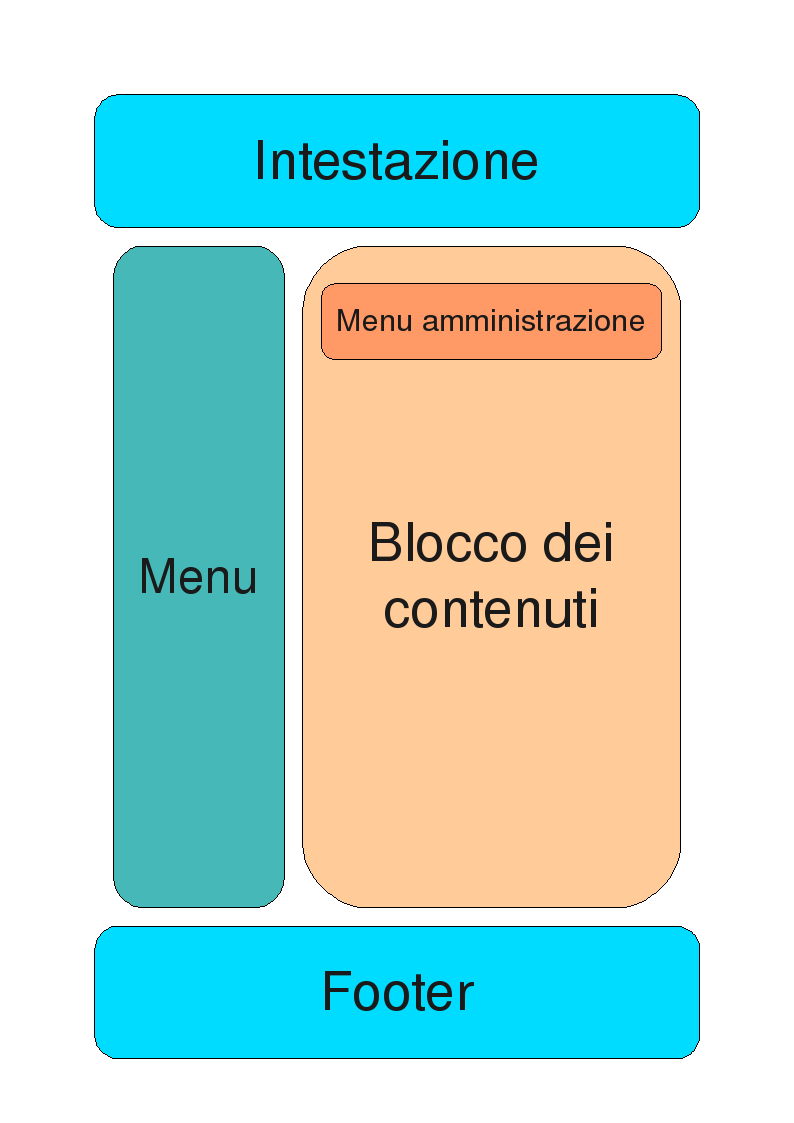
\includegraphics[scale=0.36]{images/layout.png}
\subsubsection{Templates}
Il sistema Sigeol prevede un diverso template per ogni azione raggiungibile attraverso una richiesta GET presente in ogni controller. Di seguito viene riportata una descrizione di ogni template:
\subsubsection*{Template comuni a più controller}
Per evitare fastidiose ripetizione di seguito sono riportate le descrizioni dei template per le azioni che figurano in più controller:
\begin{itemize}
 \item \verb|new.html.erb|: presenta un \underline{form} per l'inserimento di una nuova istanza.
 \item \verb|edit.html.erb|: presenta un form per la modifica di un'istanza esistente.
 \item \verb|index.html.erb|: presenta un elenco ordinato di un insieme di istanze.
 \item \verb|show.html.erb|: presenta le informazioni relativa ad una determinata istanza.
 \item \verb|administration.html.erb|: presenta un elenco ordinato di un insieme di istanza e le relative funzioni
 per amministrarle.
 \item \verb|new_constraint.html.erb|: presenta un form per l'inserimento di un nuovo vincolo o preferenza
\end{itemize}
Inoltre per garantire l'interoperabilità dei dati sono presenti i template XML per tutte le azioni \verb|index| e \verb|show|, nonchè un template PDF per l'azione \verb|show| di \verb|TimetablesController|. Infine è presente il template per la mail che sarà inviata al docente per l'attivazione del proprio user.
\subsubsection*{Template per TeachingsController}
Il template XHTML \verb|select_teacher.html.erb| è presente per il \\ \verb|TeachingsController| per l'azione \verb|select_teacher|.  Questo presenta un form per l'assegnamento di un docente ad un insegnamento utilizzando metodi per la presentazione automatica della lista dei docenti come i tag XHTML \verb|<select>| e \verb|<option>|.
\subsubsection*{Template per CurriculumsController}
Il template XHTML \verb|select_teaching.html.erb| è presente per il \\ \verb|CurriculumsController| per l'azione \verb|select_teaching|.  Questo presenta un form per l'assegnamento di un insegnamento ad un curriculum utilizzando metodi per la presentazione automatica della lista degli insegnamenti come i tag XHTML \verb|<select>| e \verb|<option>|.
\subsubsection*{Template per TeachersController}
Il \verb|TeachersController| prevede diverse azioni raggiungibili attraverso una richiesta GET ed i relativi template XHTML sono i seguenti:
\begin{itemize}
 \item \verb|pre_activate.html.erb|: presenta un form per l'attivazione dello \verb|user| del docente invitato
 \item \verb|edit_capabilities.html.erb|: presenta un form per l'assegnazione di nuovi privilegi allo \verb|user| detenuto dal docente utilizzando metodi per la presentazione automatica della lista dei privilegi come li tag XHTML \verb|<input type="checkbox">|
 \item \verb|edit_graduate_courses.html.erb|: presenta un form per l'assegnazione di nuovi corsi di laurea allo \verb|user| dtenuto dal docente utilizzando metodi per la presentazione automatica della lista dei corsi di laurea come i tag XHTML \verb|<select>| e \verb|<option>|
\end{itemize}
\subsubsection{Partials}
Il sistema Sigeol prevede l'uso di partials per la visualizzazione delle informazioni che sono riutilizzate in più view. Ognuno di essi è caratterizzato dalla presenza di un \_ (underscore) prima del nome del file che sono della forma \verb|_show_nomemodel.html.erb| e \verb|_show_nomemodel_admin.html.erb| e dovranno essere contenuti nella rispettiva directory che contiene i template del controller associato a \verb|nomemodel| (ad esempio \verb|_show_teaching.html.erb| è contenuto all'interno della directory \verb|app\views\teachings|. I partial del primo tipo visualizzano le informazioni dell'oggetto di tipo \verb|nomemodel| per le azioni di pubblico accesso, mentre i secondi per le azioni di amministrazione con le relative funzioni.

Per i controller che presentano l'azione \verb|administration| e necessitano di un menu di amministrazione è presente un partial \verb|_menu_admin.html.erb| per la visualizzazione del suddetto menu che risiederà nella stessa directory che contiene i template del controller in questione.

I partials, infine, che vengono utilizzati dal layout sono contenuti nella directory \verb|app\views\shared|, come ad esempio \verb|_user_sidebar.html.erb|.
\subsection{Componente Helper}\label{helper}
Il componente Helper si occupa di raccogliere le funzionalità di utilità necessarie ai componenti del pattern MVC. Ogni file che rappresenta un Helper non conterrà una classe, bensì un modulo, ovvero un insieme di metodi di pubblica utilità. Per ogni controller è previsto lo specifico Helper, anche se non è necessario che siano presenti dei metodi in quanto non tutti i controller (e le rispettive view) necessitano di funzioni ausiliarie.
\subsubsection{ApplicationHelper}
L' \verb|ApplicationHelper| contiene i metodi di utilità che non trovano una collocazione logica negli altri helper, nonchè tutte le funzionalità ausiliare richieste da più classi delle diverse componenti.
I metodi presenti all'interno dell' \verb|ApplicationHelper| sono i seguenti:
\begin{itemize}
 \item \verb|first_upper(name)|: metodo che restituisce la stringa \verb|name| a cui viene reso maiscolo il primo carattere e minuscoli i rimanenti.
 \item \verb|login_form|: metodo che \underline{renderizza} il partial per la form per il login.
 \item \verb|standard_sidebar|: metodo che renderizza il partial per il menu pubblico.
 \item \verb|user_sidebar|: metodo che renderizza il partial per il menu privato.
 \item \verb|link(user)|: metodo che restituisce l'insieme dei link disponibili per \verb|user|.
\end{itemize}
\subsubsection{BuildingsHelper}
I metodi presenti all'interno del \verb|BuildingsHelper| sono i seguenti:
\begin{itemize}
 \item \verb|menu_admin|: metodo che renderizza il partial per il menu di amministrazione per gli edifici.
 \item \verb|show_building_admin(building)|: metodo che renderizza il partial per l'amministrazione del \verb|building|.
 \item \verb|show_building(building)|: metodo che renderizza il partial per la visualizzazione del \verb|building|.
\end{itemize}
\subsubsection{ClassroomsHelper}
I metodi presenti all'interno del \verb|ClassroomsHelper| sono i seguenti:
\begin{itemize}
 \item \verb|menu_admin|: metodo che renderizza il partial per il menu di amministrazione per le aule.
 \item \verb|show_classroom_admin(classroom)|: metodo che renderizza il partial per l'amministrazione della \verb|classroom|.
\item \verb|show_classroom(classroom)|: metodo che renderizza il partial per la visualizzazione della \verb|classroom|.
\end{itemize}
\subsubsection{CurriculumsHelper}
I metodi presenti all'interno del \verb|CurriculumsHelper| sono i seguenti:
\begin{itemize}
\item \verb|show_curriculum_admin(curriculum)|: metodo che renderizza il partial per l'amministrazione del \verb|curriculum|.
\item \verb|show_curriculum(curriculum)|: metodo che renderizza il partial per la visualizzazione del \verb|curriculum|.
\end{itemize}
\subsubsection{SessionsHelper}
Non è presente nessun metodo all'interno di \verb|SessionsHelper|.
\subsubsection{GraduateCoursesHelper}
I metodi presenti all'interno del \verb|GraduateCoursesHelper| sono i seguenti:
\begin{itemize}
 \item \verb|menu_admin|: metodo che renderizza il partial per il menu di amministrazione per i corsi di laurea
 \item \verb|show_graduate_course_admin(graduate_course)|: metodo che renderizza il partial per l'amministrazione del  \verb|graduate_course|.
\item \verb|show_graduate_course(graduate_course)|: metodo che renderizza il partial per la visualizzazione del \verb|graduate_course|.
\end{itemize}
\subsubsection{TeachersHelper}
I metodi presenti all'interno del \verb|TeachersHelper| sono i seguenti:
\begin{itemize}
 \item \verb|menu_admin|: metodo che renderizza il partial per il menu di amministrazione per i docenti.
 \item \verb|show_teacher_admin(teacher)|: metodo che renderizza il partial per l'amministrazione del \verb|teacher|.
 \item \verb|show_teacher(teacher)|: metodo che renderizza il partial per la visualizzazione del \verb|teacher|.
\end{itemize}
\subsubsection{TeachingsHelper}
I metodi presenti all'interno del \verb|TeachingsHelper| sono i seguenti:
\begin{itemize}
 \item \verb|menu_admin|: metodo che renderizza il partial per il menu di amministrazione per gli insegnamenti.
 \item \verb|show_teaching_admin(teaching)|: metodo che renderizza il partial per l'amministrazione del \verb|teaching|.
 \item \verb|show_teaching(teaching)|: metodo che renderizza il partial per la visualizzazione del \verb|teaching|.
\end{itemize}
\subsubsection{TimetablesHelper}
I metodi presenti all'interno del \verb|TimetablesHelper| sono i seguenti:
\begin{itemize}
 \item \verb|menu_admin|: metodo che renderizza il partial per il menu di amministrazione per gli orari.
 \item \verb|show_timetable_admin(timetable)|: metodo che renderizza il partial per l'amministrazione del \verb|timetable|.
 \item \verb|show_timetable(timetable)|: metodo che renderizza il partial per la visualizzazione del \verb|timetable|.
\end{itemize}
\subsubsection{UsersHelper}
I metodi presenti all'interno del \verb|UsersHelper| sono i seguenti:
\begin{itemize}
 \item \verb|show_not_active_users(user)|: metodo che renderizza il partial per la visualizzazione dello \verb|user| non ancora attivo.
\end{itemize}
\subsection{Componente MiddleMan}
Il componente \verb|MiddleMan| viene utilizzato per effettuare esecuzioni (istantanee e/o schedulate) di calcolo dell'orario. \\ 
Esso implementa le seguenti operazioni:
\begin{itemize}
\item aggiunta di nuove date per la generazione dell'orario relativo ad uno specifico corso di laurea
\item delega alla componente \verb|Algorithm| la generazione dell'orario relativo ad uno specifico corso di laurea
\item segnala all'applicazione la fine del calcolo 
\end{itemize}
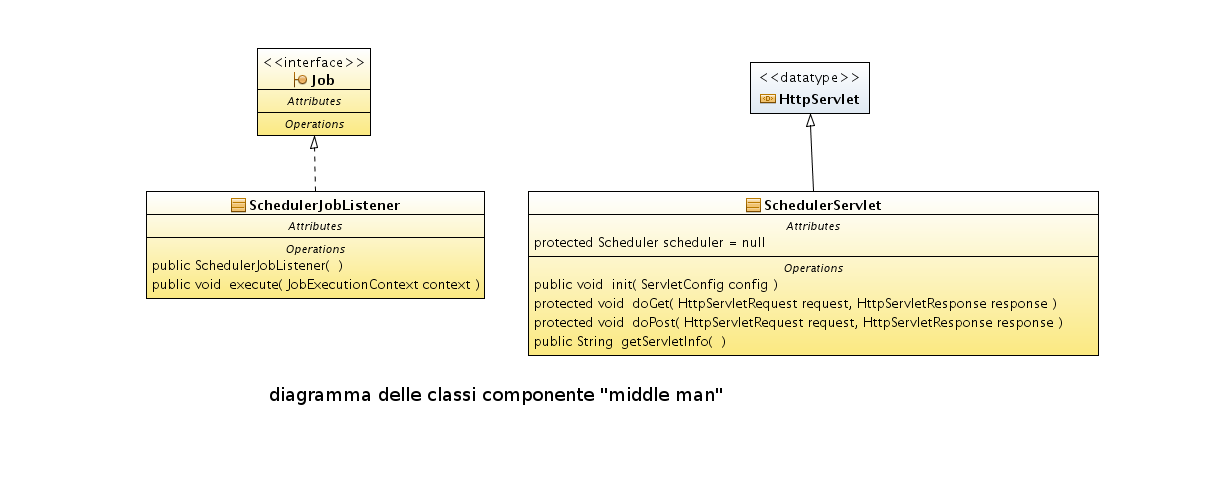
\includegraphics[scale=0.34]{images/MMserv_diagram_class.png}
\subsubsection{SchedulerServlet}
Servlet che si occupa di ricevere le richieste (di tipo HTTP POST e GET) dall'applicazione:
\begin{description}
\item[POST]
Parametri: course, date\\
crea una nuovo trigger che si attiverà alla data (date) per il corso di laurea (course) specificato 
\item[GET]
Parametri: course, inputfile, timeout\\
viene inizializzata ed eseguita la componente \verb|Algorithm| con i parametri ricevuti
\end{description}
\subsubsection{SchedulerJobListener}
Classe che viene richiamata all'attivazione di un evento precedentemente schedulato (nel nostro caso la generazione dell'orario di un determinato corso di laurea ad una certa data).
Si occupa di segnalare all'applicazione (attraverso il metodo \textbf{execute}) l'attivazione del calcolo dell'orario del corso di laurea specificato  
\subsection{Componente Algorithm}
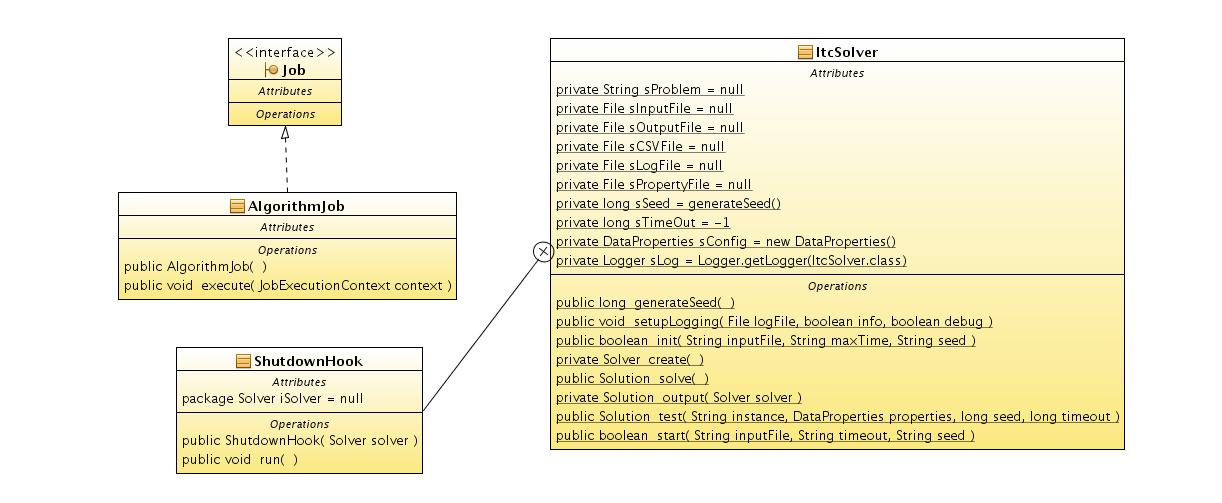
\includegraphics[scale=0.34]{images/MMalg_diagram_class.png}
\subsubsection{AlgorithmJob}
Ogni singola istanza della classe \verb|AlgorithmJob| esegue il calcolo dell'orario relativo ad un determinato corso di laurea.
\subsubsection{ItcSolver}
Classe che si occupa di leggere il file di input (contenente tutte le informazioni richieste relative al calcolo e generazione dell'orario) ed eseguire effettivamente l'algoritmo.
\subsubsection{Descrizione dell'algoritmo}
L'algoritmo utilizzato per la generazione dell'orario si basa su \verb|Constraint Solver Library| (CPSolver 1.1,  copyright (C) 2007 Tomáš Müller): tale libreria permette la modellazione di una realtà universitaria al fine di elaborare diverse tipologie di orari, in base alle necessità.
\subsubsection*{Risultati internazionali}
Il CPSolver 1.1 ha concorso nella \verb|International Timetabling Competition 2007 (ITC 2007)|: tale competizione era strutturata in 3 diverse tipologie di problemi da risolvere:
\begin{enumerate}
 \item Generazione di orari d'esame
 \item Generazione di orari di lezione basati sulla struttura del corso di laurea
 \item Generazione di orari di lezione basati sulle iscrizioni dei diversi studenti ai corsi
\end{enumerate}
L'algoritmo è giunto tra i finalisti in tutti i diversi problemi, aggiudicandosi il primo posto nelle tipologie 1 e 2 (sito web ufficiale: \textit{http://www.cs.qub.ac.uk/itc2007/index.htm}).
\subsubsection*{Motivazioni della scelta}
CPSolver 1.1 è stato scelto dal nostro team in seguito ad un'attenta analisi. Le motivazioni che ci hanno portato ad adottarlo sono riassumibili in:
\begin{itemize}
 \item Ottimi risultati a livello internazionale
 \item Totalmente open source
 \item La libreria è scritta interamente in Java, e Ruby, tramite l'implementazione JRuby, supporta in maniera eccellente Java
 \item Il codice sorgente è strutturato in maniera ordinata e corretta
 \item La documentazione relativa è ampia e facilmente accessibile
\end{itemize}
\subsubsection*{Curriculum Course Timetabling}
Il \verb|Curriculum Corse Timetabling (CCT)| rappresenta la sezione del CPSolver 1.1 che risolve il problema della generazione di orari di lezione basati sulla struttura dei corso di laurea. Qui di seguito ne verranno analizzati gli aspetti di maggiore importanza.
\paragraph{Entità coinvolte}
Le entità coinvolte  nella generazione dell'orario sono:
\begin{itemize}
 \item i corsi di laurea su cui si desidera elaborare l'orario delle lezioni
 \item gli insegnamenti appartenenti ai corsi di laurea interessati
 \item il numero dei giorni di lezione (solitamente 5)
 \item il numero di fasce orarie giornaliere
\end{itemize}
\subsubsection*{Vincoli}
I vincoli che l'algoritmo deve rispettare sono:
\begin{itemize}
 \item tutte le lezioni di un insegnamento devono essere presenti all'interno dell'orario, ed assegnate a giorni e/o fasce orarie differenti
 \item due lezioni non possono tenersi contemporaneamente nella stessa aula
 \item due lezioni non possono tenersi contemporaneamente nello stesso giorno e nella stessa fascia oraria
 \item tutte le lezioni dello stesso anno devono essere tenute in giorni e/o fasce orarie differenti, vietando sovrapposizioni 
 \item tutte le lezioni tenute dallo stesso docente devono essere tenute in giorni e/o fasce orarie differenti
 \item tutti i giorni e/o fasce orarie caratterizzati da indisponibilità devono essere rispettati/e
\end{itemize}
\subsubsection*{Fattori di scelta}
La soluzione migliore viene trovata in base ai seguenti fattori:
\begin{itemize}
 \item la capacità dell'aula preposta ad ospitare la lezione di un determinato insegnamento deve cercare di garantire il posto a sedere agli studenti previsti dall'insegnamento stesso
 \item le lezioni di un determinato insegnamento devono essere tenute almeno in un numero minimo prefissato di giorni diversi
 \item le lezioni dello stesso anno devono essere il più possibile adiacenti le une con le altre, riducendo le eventuali ore buche
 \item le lezioni dello stesso insegnamento devono essere tenute il più possibile nella stessa aula
 \item le preferenze sui singoli insegnamenti devono essere il più possibile rispettate
\end{itemize}
\subsubsection*{Componenti interne}
Tutte le informazioni relative a CPSolver 1.1, compresa la relativa documentazione, sono reperibili all'indirizzo: \textit{http://cpsolver.sourceforge.net/api/index.html}.

La versione originale dell'algoritmo permette la sola gestione dei vincoli. Al fine di garantire un prodotto il più possibile adattabile alle diverse realtà universitarie, il team QuiXoft ha innestato all'interno della libreria la gestione delle preferenze sui singoli insegnamenti. Tali modifiche sono state apportate nel modo meno invasivo possibile, lasciando il più incontaminato possibile il codice sorgente originale.

Prima di continuare la trattazione delle componenti occorre rendere nota la seguente convenzione in uso da parte del CPSolver 1.1 e che è stata mantenuta durante il nostro sviluppo:
\begin{itemize}
 \item i giorni interessati nella generazione dell'orario vengono individuati tramite valore numerico: ove N°Giorni rappresenta il numero dei giorni di lezione, 0,1, .. N°Giorni-1 rappresentano in formato numerico i giorni di interesse. Ipotizzando, ad esempio, 5 giorni a disposizione: 0 = LUN, 1 = MAR, .. , 4 = VEN
 \item le fasce orarie vengono individuate tramite valore numerico: ove N°FasceOrarie rappresenta il numero di fasce orarie giornaliere, 0,1 .. N°FasceOrarie rappresentano in formato numerico le fasce orarie. Ipotizzando, ad esempio, 6 fasce orarie: 0 = 1° fascia, 1 = 2°fascia, .. , 5 = 6°fascia
\end{itemize}
I nomi delle classi e dei metodi rispecchiano le convenzioni standard di Java. La lingua di riferimento adottata, come nel CPSolver 1.1,  è la lingua inglese, commenti compresi.
\subsubsection*{La classe MyPreferences\_DaySlot}
La classe \verb|MyPreferences_DaySlot| rappresenta il gestore delle preferenze. Le preferenze che gestisce sono relative ad un insegnamento, in particolare rappresentano i giorni e/o le fasce orarie in cui tale insegnamento non è desiderabile venga tenuto. 
L'insieme delle preferenze è organizzato sotto forma di \verb|Vector| (\textit{http://java.sun.com/j2se/1.4.2/docs/api/java/util/Vector.html}), il cui tipo base è \verb|DaySlot_PreferenceInfo|.
\subsubsection*{La classe interna DaySlot\_PreferenceInfo}
La classe \verb|DaySlot_PreferenceInfo| rappresenta una singola preferenza. Ogni preferenza è caratterizzata da diverse informazioni quali:
\begin{itemize}
\item	il codice identificativo dell'insegnamento a cui essa fa riferimento
\item	il giorno e la fascia oraria in cui è desiderabile non venga tenuto l'insegnamento
\item	il peso della preferenza stessa
\end{itemize}
Il peso rappresenta un valore numerico attraverso il quale si assegna un valore di importanza ad una preferenza. Tale peso permette all'algoritmo di tenere in maggiore considerazione le preferenze ``molto desiderabili'', rispetto, ad esempio, a preferenze minori.

\paragraph{Pesi e priorità delle preferenze}
L'assegnazione dei pesi viene gestita internamente alla classe in base ad una scala di priorità. I valori dei pesi sono stati scelti dal team QuiXoft in modo da garantire una corretta ed efficiente elaborazione. La relazione tra il valore di priorità ed il peso che tale priorità associa alla preferenza è riassumibile con la tabella seguente:

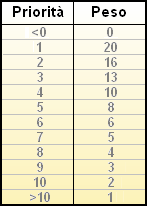
\includegraphics[scale=1]{images/Algoritm_WeightPriorityRelation.png}
\subsubsection*{I metodi}
I metodi privati presenti all'interno della classe \verb|MyPrefereces_DaySlot| sono:
\begin{itemize}
\item \verb|int getWeightFromPriority (int)| : in base al valore di priorità restituisce il peso corrispondente secondo la tabella precedente.
\item \verb|DaySlot_PreferenceInfo getPreference (String, int, int)| : restituisce un riferimento alla preferenza di uno specifico insegnamento, in base al giorno ed alla fascia oraria di interesse. Nel caso in cui tale preferenza non esistesse il valore restituito è \verb|null|.
\item \verb|bool existsCoursePreference (String)| : in base al codice identificativo di un insegnamento, restituisce TRUE se esiste almeno una preferenza relativa allo stesso, FALSE nel caso in cui non ne esista alcuna. 
\end{itemize}

I metodi pubblici messi a disposizione sono:
\begin{itemize}
\item \verb|addPreference(String, int, int, int)| : aggiunge una preferenza all'insieme delle preferenze. I parametri formali rappresentano l'identificativo dell'insegnamento, il giorno e la fascia oraria in cui è desiderabile non venga tenuta alcuna lezione dell'insegnamento specificato, ed il valore di priorità che la preferenza assumerà all'interno del sistema di calcolo.
\item \verb|getPreferencesPenality(String)| : restituisce il valore di penalità associato ad un determinato insegnamento. I valore di penalità viene calcolato in base alle preferenze non soddisfatte.
\end{itemize}
\subsubsection*{Dati di input}\label{Algo_Input}
Per quanto riguarda l'input, l'algoritmo si basa su un file con estensione \verb|.cct| (Curriculum Course Timetabling) il quale contiene i dati necessari all'elaborazione dell'orario delle lezioni.

La struttura interna del file di input è definibile attraverso le diverse sezioni che la compongono; più precisamente esse sono:
\begin{itemize}
\item	Sezione \verb|MODEL|: informazioni generali
\item	Sezione \verb|COURSES|: elenco dei vari insegnamenti
\item	Sezione \verb|ROOMS|: elenco delle aule
\item	Sezione \verb|CURRICULA|: elenco dei relativa corsi di laurea
\item	Sezione \verb|UNAVAIBILITY_CONSTRAINTS|: elenco delle indisponibilità
\item	Sezione \verb|PREFERENCES|: elenco delle preferenze
\end{itemize}
La sezione \verb|MODEL| rappresenta il preambolo del file. Tratta le informazioni di carattere generale riguardanti la realtà universitaria sulla quale si genererà l'orario delle lezioni. Si suddivide nei seguenti campi:
\begin{itemize}
\item	\verb|Name|: indica il nome della realtà di riferimento
\item	\verb|Courses|: indica il numero complessivo dei corsi 
\item	\verb|Rooms|: indica il numero delle aule a disposizione
\item	\verb|Days|: indica il numero di giorni di lezione
\item	\verb|Periods_per_day|: indica il numero di fasce orarie in cui è suddiviso ogni giorno
\item	\verb|Curricula|: indica il numero dei corsi di laurea e relativi curricula interessati nella generazione dell'orario
\item	\verb|Constraints|: indica il numero di vincoli di indisponibilità
\end{itemize}

Per la trattazione delle sezioni seguenti occorre avvalersi della seguente convenzione:
\begin{itemize}
\item il carattere | indica la divisione dal campo precedente al successivo, e corrisponde al carattere \verb|blank| nel file reale
\item i campi preceduti dal carattere \# indicano campi a cui è assegnata un'informazione di tipo numerico
\end{itemize}

La sezione \verb|COURSES| identifica la sezione nella quale vengono elencati tutti gli insegnamenti e relative caratteristiche. Ogni riga di questa sezione rappresenta un singolo corso, e si attiene alla struttura seguente: \begin{verbatim}
 CourseID | Teacher | #Lectures | MinWorkingDays | #Students
\end{verbatim}

La sezione \verb|ROOMS| identifica la sezione nella quale vengono elencate tutte le aule a disposizione e relativa capacità. Ogni riga di questa sezione rappresenta una singola aula, e si attiene alla  struttura seguente:
\begin{verbatim}
 RoomID | #Capacity
\end{verbatim}

La sezione \verb|CURRICULA| identifica la sezione nella quale vengono elencati tutti i corsi di laurea con i relativi curricula ed i relativi insegnamenti che ne fanno parte. Ogni riga di questa sezione rappresenta un singolo corso di laurea, e si attiene alla struttura seguente:
\begin{verbatim}
 CurriculumID | #Courses | CourseID ... CourseID
\end{verbatim}

La sezione \verb|UNAVAILABILITY_CONSTRAINTS| identifica la sezione nella quale vengono elencati tutti i vincoli di indisponibilità degli insegnamenti. Ogni riga di questa sezione rappresenta un singolo vincolo, e si attiene alla struttura seguente:
\begin{verbatim}
 CourseID | #Day | #TimeSlot
\end{verbatim}


La sezione \verb|PREFERENCES| identifica la sezione nella quale vengono elencate tutte le preferenze degli insegnamenti: rappresentano quando non è desiderabile venga tenuta una lezione di un determinato insegnamento. Ogni riga di questa sezione rappresenta una singola preferenza, e si attiene alla struttura seguente:
\begin{verbatim}
 CourseID | #Day | #TimeSlot
\end{verbatim}

\subsubsection*{Dati di output}
Per quanto riguarda l'output l'algoritmo produce un file che rappresenta l'intero orario delle lezioni. Ogni riga rappresenta una singola lezione, e si attiene alla struttura seguente:
\begin{verbatim}
 CourseID | RoomID | #Day | #TimeSlot
\end{verbatim}

I valori identificativi dell'insegnamento (\verb|CourseID|) e dell'aula (\verb|RoomID|) derivano dai valori delle sezioni \verb|COURSES| e \verb|ROOMS| trattate nella sezione \ref{Algo_Input}
\section{Organizzazione delle directories}
Per facilitare la comprensione dell'organizzazione del sistema Sigeol, viene presentata in questa sezione la struttura delle directories. Per un dettaglio maggiore dell'organizzazione si prega di far riferimento al sito ufficiale di Ruby on Rails. Nella figura che segue viene illustrata la gerarchia \\
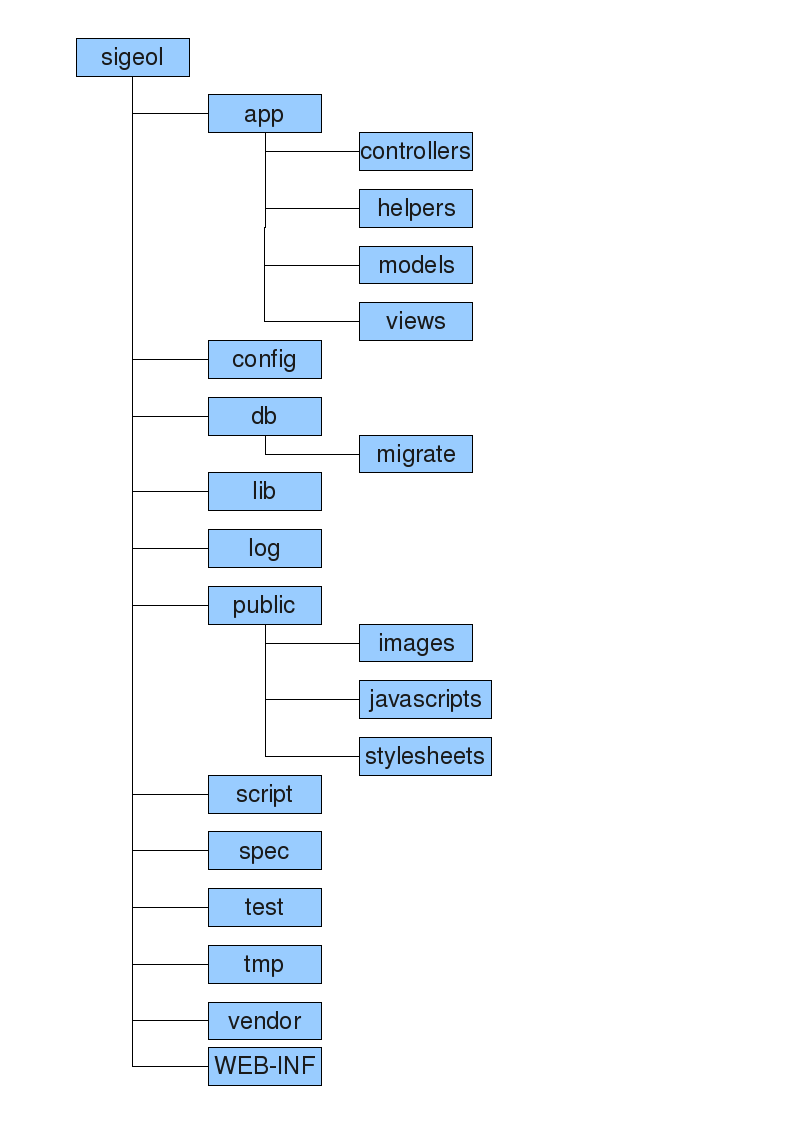
\includegraphics[scale=0.59]{images/gerarchiacartelle.png} \\
A differenza delle consuete applicazioni sviluppate tramite il framework Rails, il sistema Sigeol presenta la cartella \verb|WEB-INF| che contiene tutte le classi e librerie utilizzate dalla servlet e il suo file di configurazione web.xml.\\ Per ulteriori informazioni sulla tecnologia servlet visitare il sito \\ http://java.sun.com/products/servlet/ .
\section{Tracciamento componenti-requisiti}
Di seguito è riportato il tracciamento dei requisiti descritti nel documento denominato \textsc{Analisi dei Requisiti} con le componenti descritti nel presente.\\
\begin{center}
\begin{small}
\begin{tabular}{|c||c|c|c|c|c|}
\hline
\textsc{Requisiti} & \textsc{View} & \textsc{Controller} & \textsc{Model} & \textsc{MiddleMan} & \textsc{Algorithm}\\ \hline \hline
RFO0.0 & \checkmark & \checkmark & \checkmark & & \\
\hline
RFO0.1 & \checkmark & \checkmark & \checkmark & & \\
\hline
RFO0.2 & \checkmark & \checkmark & \checkmark & & \\
\hline
RFO0.3 & \checkmark & \checkmark & \checkmark & & \\
\hline
RFO0.4 & \checkmark & \checkmark & \checkmark & & \\
\hline
RFO0.5 & \checkmark & \checkmark & \checkmark & & \\
\hline
RFO0.6 & \checkmark & \checkmark & \checkmark & & \\
\hline
RFO0.7 & \checkmark & \checkmark & \checkmark & \checkmark & \checkmark \\
\hline
RFO0.8 & \checkmark & \checkmark & \checkmark & & \\
\hline
RFO0.9 & \checkmark & \checkmark & \checkmark & & \\
\hline
RFO0.10 & \checkmark & \checkmark & \checkmark & & \\
\hline
RFO0.11 & \checkmark & \checkmark & \checkmark & & \\
\hline
RFO0.12 & \checkmark & \checkmark & \checkmark & & \\
\hline
RFO0.13 & \checkmark & \checkmark & \checkmark & & \\
\hline
RFO0.14 & \checkmark & \checkmark & \checkmark & & \\
\hline
RFO0.15 & \checkmark & \checkmark & \checkmark & & \\
\hline
RFO0.16 & \checkmark & \checkmark & \checkmark & & \\
\hline
RFO0.17 & \checkmark & \checkmark & \checkmark & & \\
\hline
RFO0.18 & \checkmark & \checkmark & \checkmark & & \\
\hline
RFO0.19 & \checkmark & \checkmark & \checkmark & & \\
\hline
RFO0.20 & \checkmark & \checkmark & \checkmark & & \\
\hline
RFO0.21 & \checkmark & \checkmark & \checkmark & & \\
\hline
RFO0.22 & \checkmark & \checkmark & \checkmark & & \\
\hline
RFO0.23 & \checkmark & \checkmark & \checkmark & & \\
\hline
RFO0.24 & \checkmark & \checkmark & \checkmark & & \\
\hline
\end{tabular}
\end{small}
\end{center}
\begin{center}
\begin{small}
\begin{tabular}{|c||c|c|c|c|c|}
\hline
\textsc{Requisiti} & \textsc{View} & \textsc{Controller} & \textsc{Model} & \textsc{MiddleMan} & \textsc{Algorithm}\\ \hline \hline
RFO1.0 & \checkmark & \checkmark & \checkmark & & \\
\hline
RFO1.1 & \checkmark & \checkmark & \checkmark & & \\
\hline
RFO1.2 & \checkmark & \checkmark & \checkmark & & \\
\hline
RFO1.3 & \checkmark & \checkmark & \checkmark & & \\
\hline
RFO1.4 & \checkmark & \checkmark & \checkmark & & \\
\hline
RFO1.5 & \checkmark & \checkmark & \checkmark & & \\
\hline
RFO1.6 & \checkmark & \checkmark & \checkmark & & \\
\hline
RFD0.0 & \checkmark & \checkmark & \checkmark & & \\
\hline
RFD0.1 & \checkmark & \checkmark & \checkmark & & \\
\hline
RFD0.2 & & & \checkmark & \checkmark & \\
\hline
RFD0.3 & \checkmark & \checkmark & \checkmark & & \\
\hline
RFD1.0 & \checkmark & \checkmark & \checkmark & & \\
\hline
RFD2.0 & \checkmark & \checkmark & \checkmark & & \\
\hline
RFD2.1 & \checkmark & \checkmark & \checkmark & & \\
\hline
RQO0 & \checkmark & & & & \\
\hline
RQO1 & & & \checkmark & & \\
\hline
RQO2 & & \checkmark & \checkmark & & \\
\hline
RQO3 & \checkmark & \checkmark & \checkmark & \checkmark & \checkmark \\
\hline
RQO4 & \checkmark & & & & \\
\hline
RQO5 & \checkmark & & & & \\
\hline
RQO6 & \checkmark & \checkmark & \checkmark & \checkmark & \checkmark \\
\hline
RQD1 & & \checkmark & \checkmark & & \\
\hline
RIO0.0 & & & \checkmark & & \\
\hline
RIO1.0 & \checkmark & \checkmark & \checkmark & & \\
\hline
RIO1.1 & \checkmark & \checkmark & \checkmark & & \\
\hline
RIO1.2 & \checkmark & & & & \\
\hline
RID0.0 & \checkmark & \checkmark & \checkmark & \checkmark & \checkmark \\
\hline
\end{tabular}
\end{small}
\end{center}
\medskip

\modifiche
\end{document}
